\documentclass[ALICE,manyauthors]{cernphprep}

\usepackage[comma,square,numbers,sort&compress]{natbib}
\usepackage{hyperref}
\usepackage{lineno}
\usepackage{subfigure}
\usepackage[section]{placeins}
\usepackage {multicol}% Multi column in the table
\usepackage {multirow}% Multi row in the table
\usepackage {units}
\usepackage {array}
\usepackage {xcolor}
\usepackage{comment}
\linenumbers

\input{commands.tex}
\begin{document}

%%%%%%%%%%%%%%%  Title page %%%%%%%%%%%%%%%%%%%%%%%%
\begin{titlepage}

\PHyear{}
\PHnumber{2021-xxx}      % required, will be obtained from PH
%\PHdate{Day Month}  % required, will be obtained from PH
\PHdate{\today}
%

%%% Put your own title + short title here:
\title{Observation of abnormal suppression of $\mathrm{f}_{0}$(980) production \\in p--Pb collisions at $\snn$ = 5.02~TeV }

\ShortTitle{}   % appears on right page headers

%%% Do not change the next lines
%\Collaboration{ALICE Collaboration\thanks{See Appendix~\ref{app:collab} for the list of collaboration members}}
\ShortAuthor{ALICE Collaboration} % appears on left page headers, do not change

\begin{abstract}
The dependence of $\mathrm{f}_{0}$(980) production on the final-state charged-particle multiplicity in p--Pb collisions at $\sqrt{s_{\mathrm{NN}}} = 5.02$~TeV with ALICE is reported. The production of $\mathrm{f}_{0}$(980) is measured via the $\mathrm{f}_0 (980) \rightarrow \pi^{+}\pi^{-}$ decay channel in a midrapidity region of $-0.5<y<0$. Particle yield ratios of $\mathrm{f}_{0}$(980) to $\pi$ and \kstar~are found to be decreasing with an increasing charged-particle multiplicity. The suppressions of the particle yield ratios of $\mathrm{f}_{0}$(980) to $\pi$ and \kstar~exhibit different $p_{\mathrm{T}}$ dependencies, suggesting different mechanisms for the observed suppression. Furthermore, the nuclear modification factor $Q_{\mbox{pPb}}$ ($R_{\mbox{pPb}}$ in centrality intervals due to the possible bias in the determination of centrality) is measured in various multiplicity ranges. The $Q_{\mbox{pPb}}$ shows strong suppression in the  $p_{\mathrm{T}}$ region up to about 4~GeV/$c$. The results on the particle yield ratios and $Q_{\mbox{pPb}}$ for $\mathrm{f}_{0}$(980) may help to understand the late hadronic phase in p--Pb collisions and the nature of the internal structure of $\mathrm{f}_{0}$(980) particles.



\color{black}

\end{abstract}
 
\end{titlepage}

\setcounter{page}{2}

% !TEX root = paper.tex

\section{Introduction}

Quantum chromodynamics (QCD), describing the strong interaction, predicts a deconfined phase of matters, quark-gluon plasma (QGP) in extremely high temperature and energy density. Such conditions are achieved with ultra-relativistic collisions of heavy-ions at the Large Hadron Collider (LHC)~\cite{Wolschin:2020qxa}. And many observations such as flow modulations~\cite{Bhalerao:2020ulk, ALICE:2019zfl}, jet quenching~\cite{ALICE:2019qyj}, and nuclear modification factors~\cite{ALICE:2019hno} support the existence of QGP~\cite{Adams:2005dq} so far.

Among many observations stating the existence of QGP is the nuclear modification factor. The nuclear modification factors for different particles in heavy-ion collisions show many particles are strongly modified as they interact with hot and dense medium. The nuclear modification factor, on the other hand, in p--A collisions~\cite{ALICE:2016dei} is measured as unity and this states that there is no strong modification in p--A collisions at high $p_{\rm{T}}>$~3~GeV/$c$.

The short-lived resonances such as $K^{*}$(892)~\cite{ALICE:2019etb, ALICE:2016sak}, $\rho$(770)~\cite{ALICE:2018qdv}, and $\Lambda$(1520)~\cite{ALICE:2018ewo} are good probes to study the properties of the dynamic evolution of the fireball~\cite{Bierlich:2021poz}. The evolution time from chemical freeze out to kinetic freeze out is comparable with the lifetime of resonances~\cite{ALICE:2011dyt, ALICE:2019xyr}. The daughter particles from them can actively interact with the hadronic gas, resulting in modifications of resonance yields. Such modifications can be observed by comparing the yield of resonances with the yield of long-lived or ground state particles~\cite{ALICE:2018pal}. Measurements of $\rho/\pi$ and $K^{*}/K$ yield ratios are good examples to study the properties of the late hadronic phase after chemical freeze out.

Light scalar mesons, whose spin, parity, and charge are zero, even, and $J^{PC} = 0^{++}$, are of particular interesting as their natures can be explained with an exotic structure~\cite{ParticleDataGroup:2020ssz}. The understanding of them lies in a long-standing puzzle, where many discussions can be found in~\cite{ExHIC:2010gcb, Jaffe:1976ig, Maiani:2004uc}. Among the mesons, \fzero~,one of scalar mesons, is observed many years ago in $\pi\pi$ scattering experiments~\cite{Mennessier:2010xz}. Despite a long history of experimental observation and theoretical research, the nature of such a short-lived resonance is not understood and there is no consensus on its internal structure, where the structure is suggested to be normal $q\bar{q}$~\cite{Chen:2003za}, compact tetraquark~\cite{Achasov:2020aun}, or $K\overline{K}$ molecule~\cite{Ahmed:2020kmp}. Moreover, \fzero~production is also interesting due to the short lifetime~\cite{ParticleDataGroup:2020ssz}, which is a good tool to study the hadronic final state and the particle formation procedure. One of models predicting the particle formation is the Canonical Statistical Model (CSM)~\cite{Vovchenko:2019kes}, which considers system-size dependent hadrochemistry at vanishing baryon density with local conservation of electric charged, baryon density, and strangeness, while allowing for undersaturation of strangeness.

The number of constituent quarks (NCQ)~\cite{Fries:2003vb} can be suggested by measuring the flow modulations and the nuclear modification factor for different particle. The elliptic flows scaled down by the NCQ are comparable between different mesons and baryons~\cite{Wang:2022det}. Application of the NCQ scaling to \fzero~is expected to provide insights into the nature of \fzero. The nuclear modification factors for baryons exhibit strong enhancement at intermediate $p_{\mathrm{T}}$ (2~$<p_{\mathrm{T}}<$~5~GeV/$c$) compared with one for meson which is mainly due to the NCQ~\cite{Cronin:1974zm}. Measurement of the nuclear modificaction factor for \fzero, therefore, can suggest the internal structure of \fzero.

In this paper, multiplicity dependent observation of abnormal suppression of \fzero~production in p--Pb collisions at $\snn$ = 5.02~TeV is reported. Measurement of \fzero~is conducted at midrapidity (-0.5~$<\mathrm{y}<$~0) for the 0~$<p_{\mathrm{T}}<$~8~GeV/$c$ range in different multiplicity classes. In Sec.~\ref{sec:setup}, ALICE apparatus is described, and the reconstruction of \fzero~and correction is explained in Sec.~\ref{sec:ana}. Systematic study for the measurement and corresponding systematic uncertainty is reported in Sec.~\ref{sec:syst}. In Sec.~\ref{sec:results}, $p_{\mathrm{T}}$ spectrum, particle yield ratios, and the nuclear modification factors are discussed and compared with model descriptions, and conclusions is given in Sec.~\ref{sec:summary}.

\label{sec:intro}






\section{Experimental setup}
\label{sec:setup}
The analyzed minimum bias events are p--Pb collisions at $\snn$~=~5.02~TeV, which are recorded by the ALICE detector during 2016. The entire subsystem of the ALICE detector is described in \cite{Carminati:2004fp, Abelev:2014ffa} at the LHC Run 2 period. The present analysis is carried out with the V0~\cite{ALICE:2013axi}, the Zero Degree Calorimeter (ZDC)~\cite{Cortese:2019nnv}, the Inner Tracking System (ITS)~\cite{ALICE:2010tia}, the Time-Of-Flight (TOF)~\cite{Jacazio:2018slq}, and the Time Projection Chamber (TPC)~\cite{Alme:2010ke} detectors.

The V0 detector has two stations located at both sides of the interaction point, V0A and V0C, each made of 32 plastic scintillator strips, covering the full azimuthal angle within the pseudorapidity intervals $2.8 < \eta < 5.1$ and $-3.7 < \eta < -1.7$, respectively. For triggering p--Pb collisions, V0A, detector on Pb-going side, is used to provide a minimum bias (MB) trigger. The V0 provides the multiplicity class using the sum of the V0A signals. The collected data samples from the minimum bias trigger corresponds to integrated luminosity of 0.24~nb$^{-1}$~\cite{ALICE:2014gvw}. The ZDC, which detects ``slow'' nucleons at very large $\eta$~\cite{Cortese:2019nnv},  also defines multiplicity class for the event selection.

The primary vertex position is reconstructed using the measured signals in the Silicon Pixel Detector (SPD)~\cite{Santoro2009:ALICESPD}, which is innermost two layers of the ITS. Reconstructed primary vertex is required to be within 10~cm from the center of the detector along the beam direction. The probability of pileup events is 0.5\% in MB events. Pileup events are rejected if the longitudinal displacement of their reconstructed vertices is larger than 0.8~cm. The TPC is the main tracking detector of ALICE, covering a pseudorapidity range of $|\eta|<$~0.9 over the full azimuth in a uniform solenoidal magnetic field of 0.5~T along the beam axis. The TPC can reconstruct charged tracks originating from the primary vertex down to $p_{\rm{T}}~$0.1~GeV/$c$. Particle identification (PID) can be done with the TPC and the TOF. The TPC measures ionization energy loss $\mathrm{d}E/\mathrm{d}x$ of charged tracks to separate particle species. The TOF helps the PID capabilities of the TPC by measuring the flight time of charged particles from the interaction point in the TPC to the TOF.

\section{Data analysis}
\label{sec:ana}
\begin{figure}[hbt!]
	\centering
	\subfigure{ 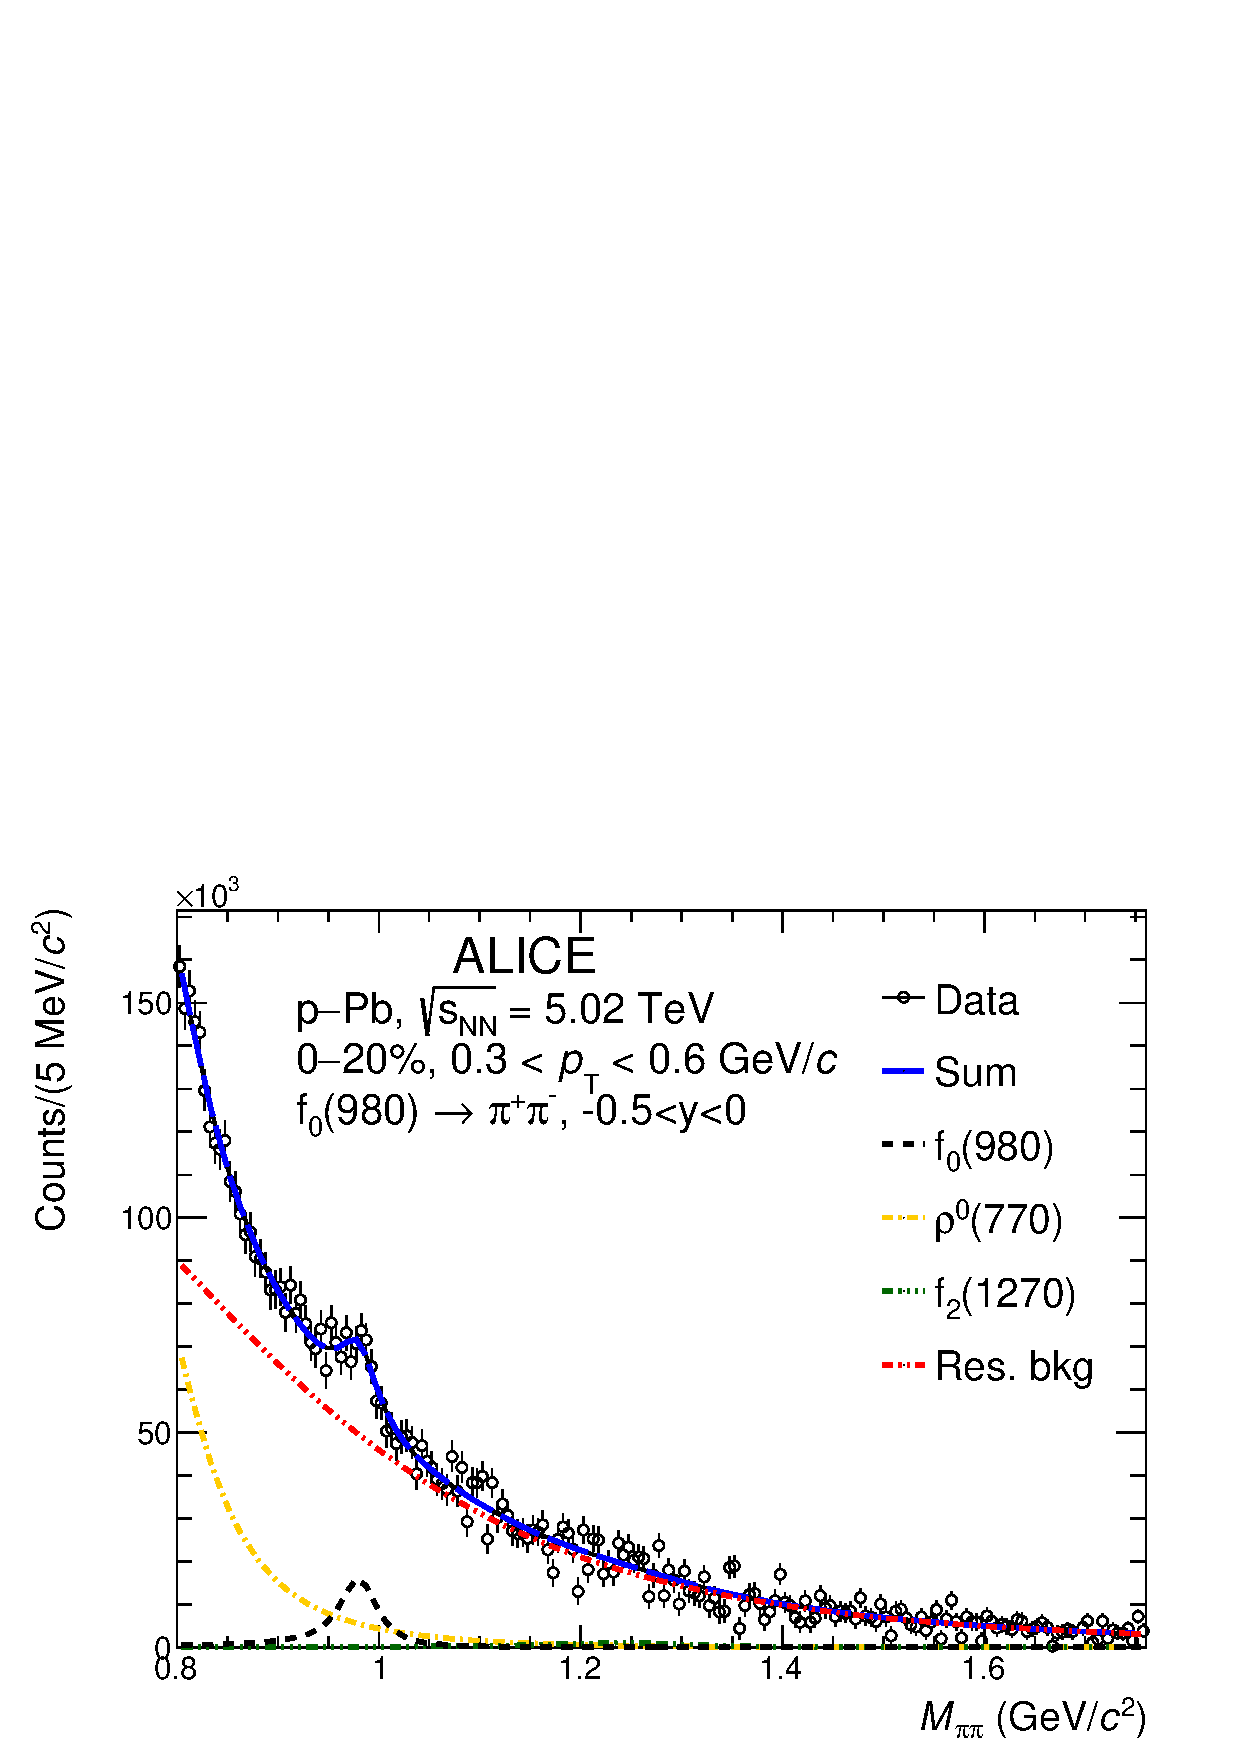
\includegraphics[width=0.47 \textwidth]{figures/Fig1_sigext_high_0pt.pdf} }
	\subfigure{ 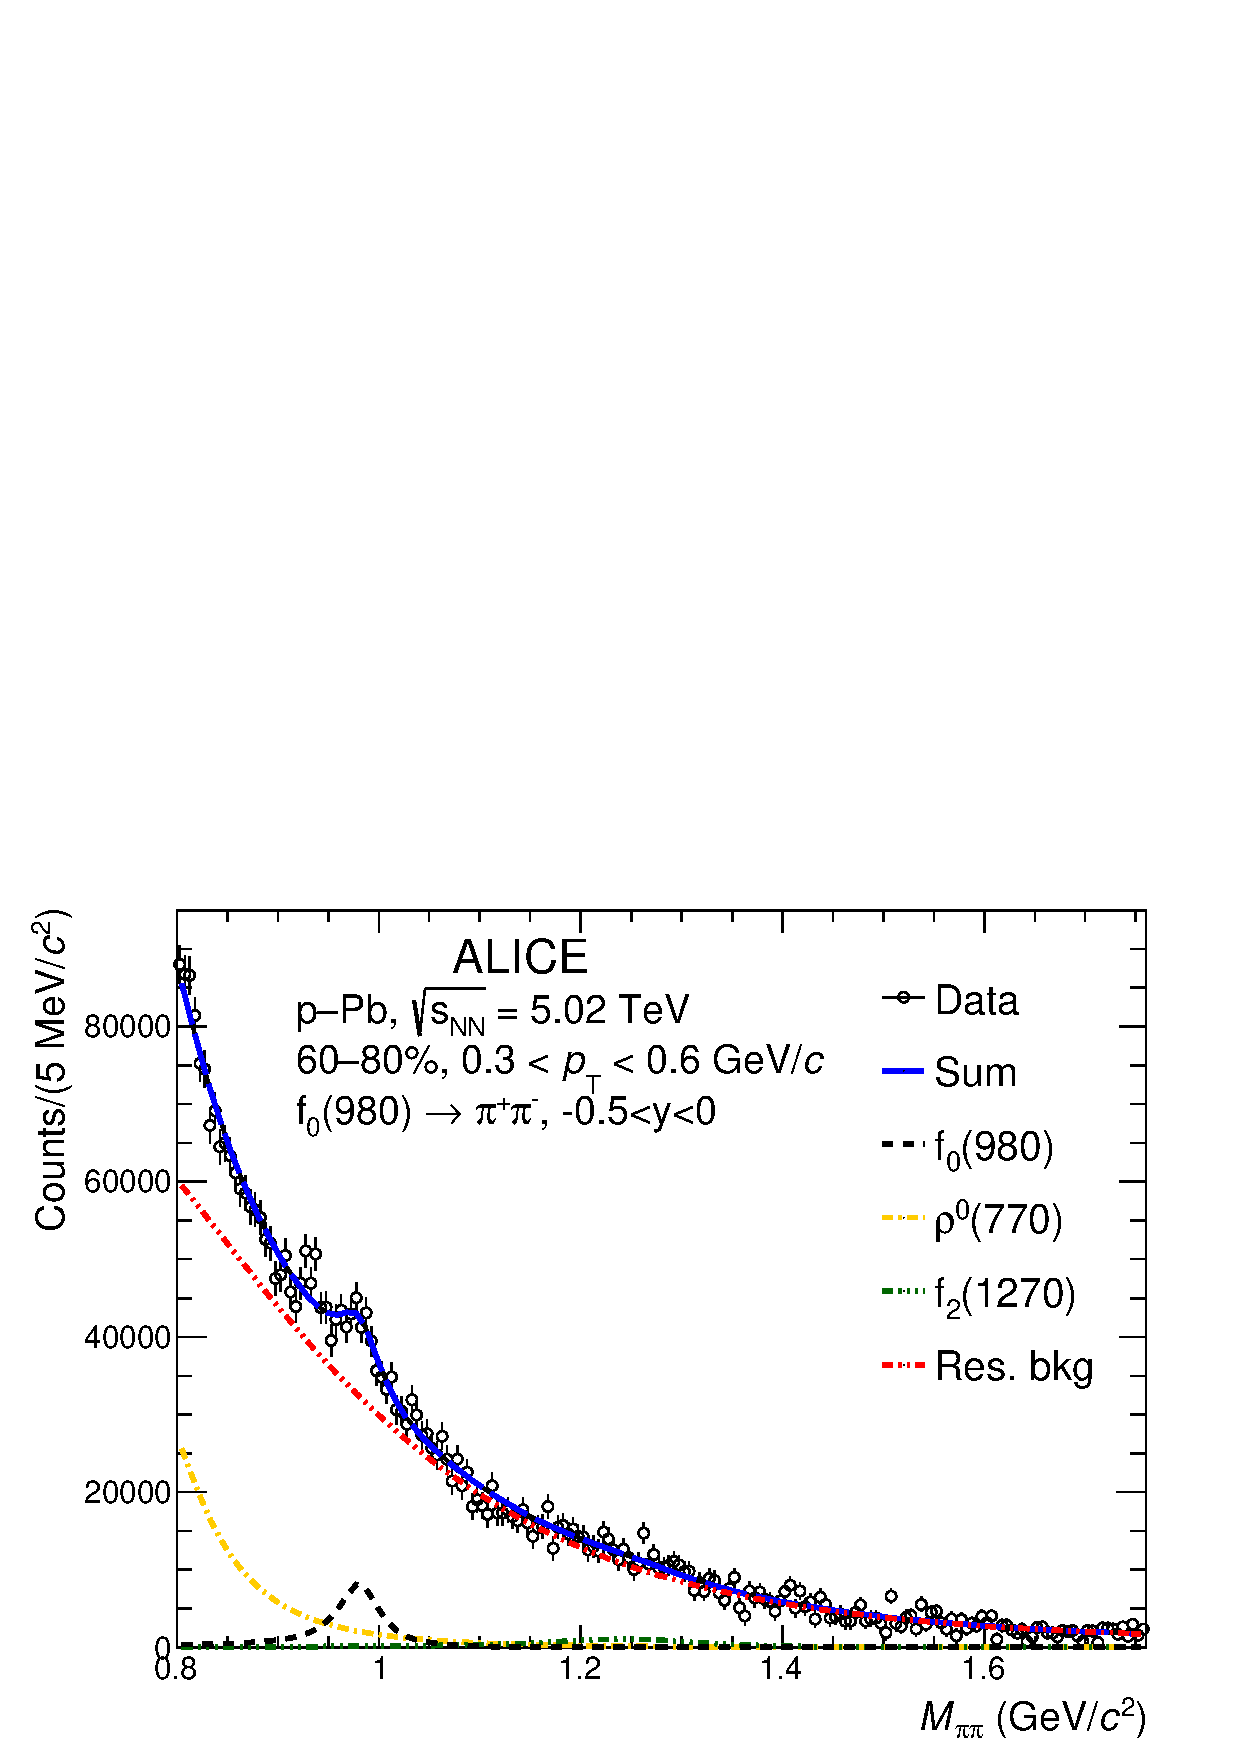
\includegraphics[width=0.47 \textwidth]{figures/Fig1_sigext_low_0pt.pdf} }
	
	\subfigure{ \includegraphics[width=0.47 \textwidth]{figures/Fig1_sigext_high_1pt.pdf} }
	\subfigure{ 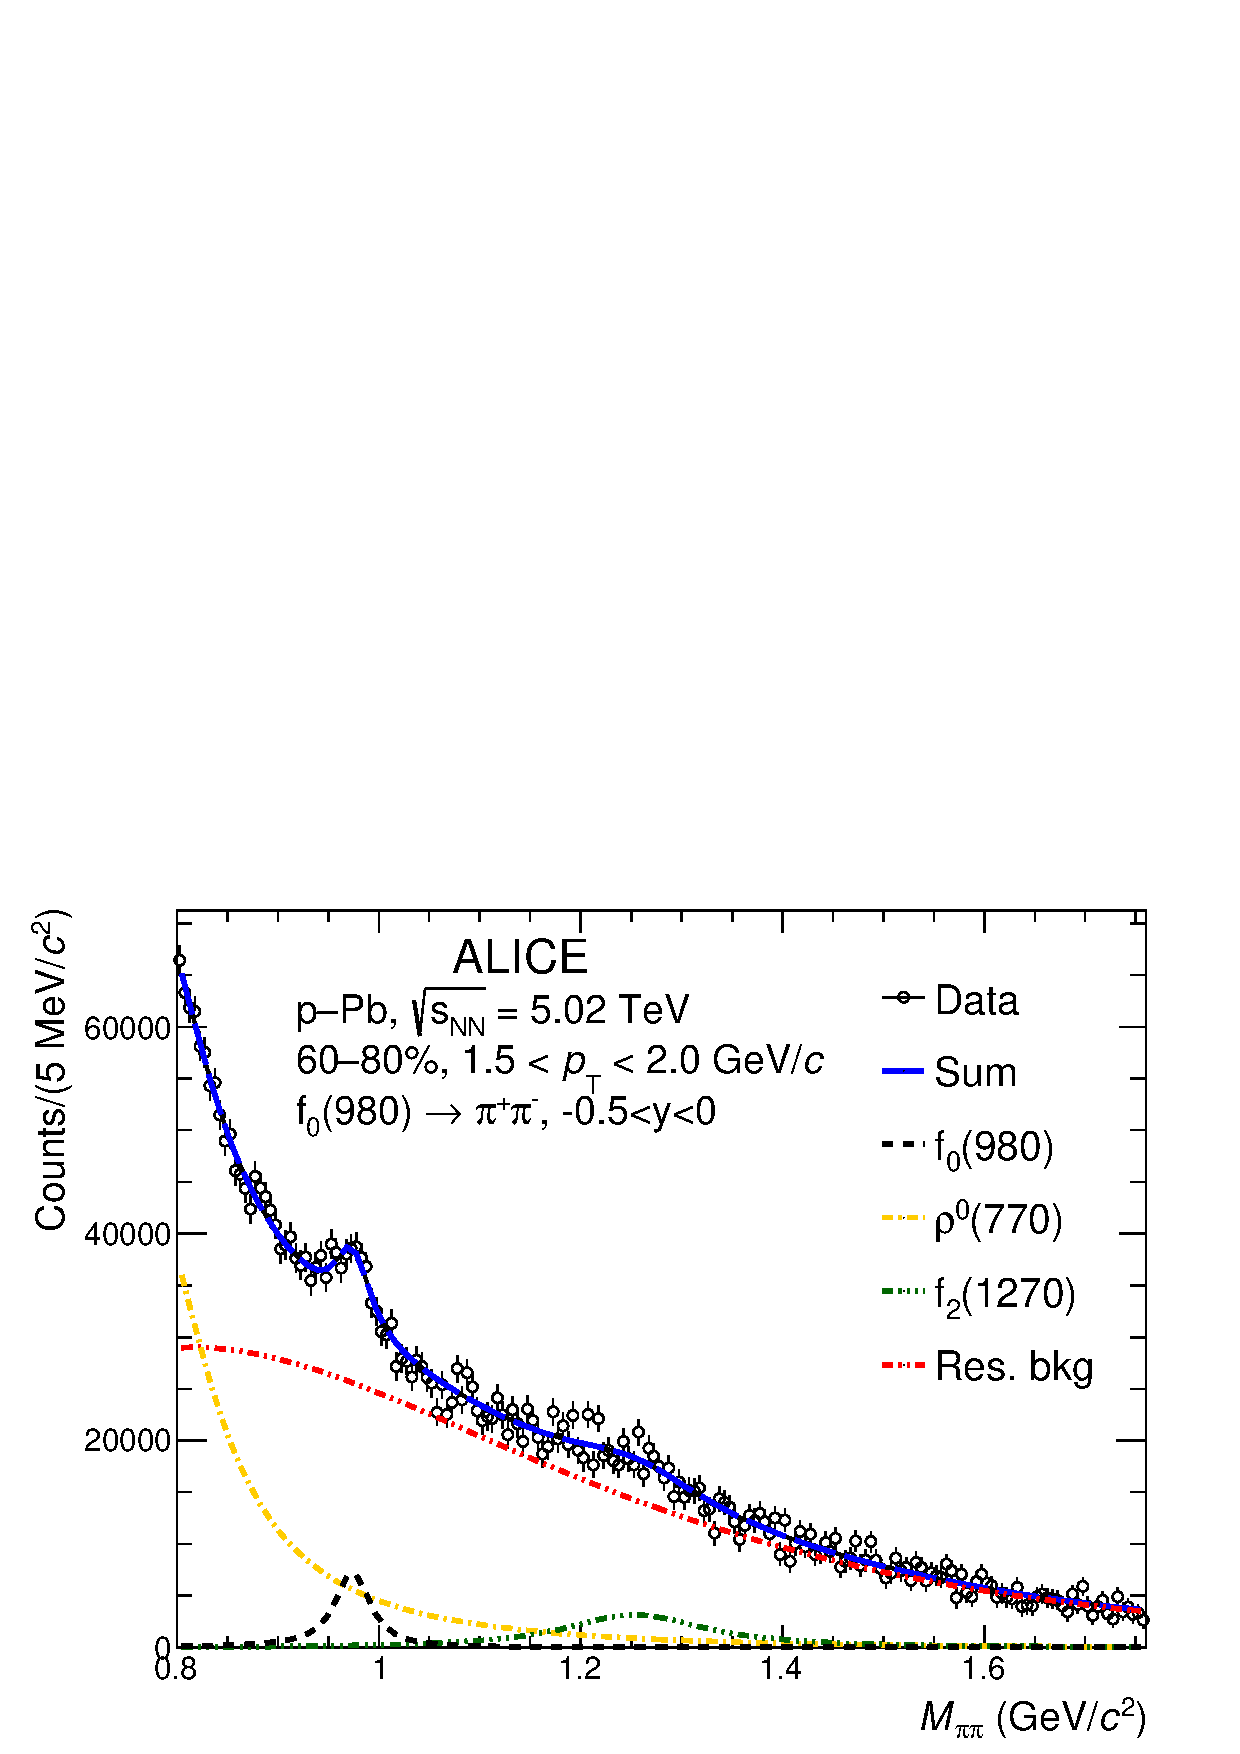
\includegraphics[width=0.47 \textwidth]{figures/Fig1_sigext_low_1pt.pdf} }
	
	\subfigure{ 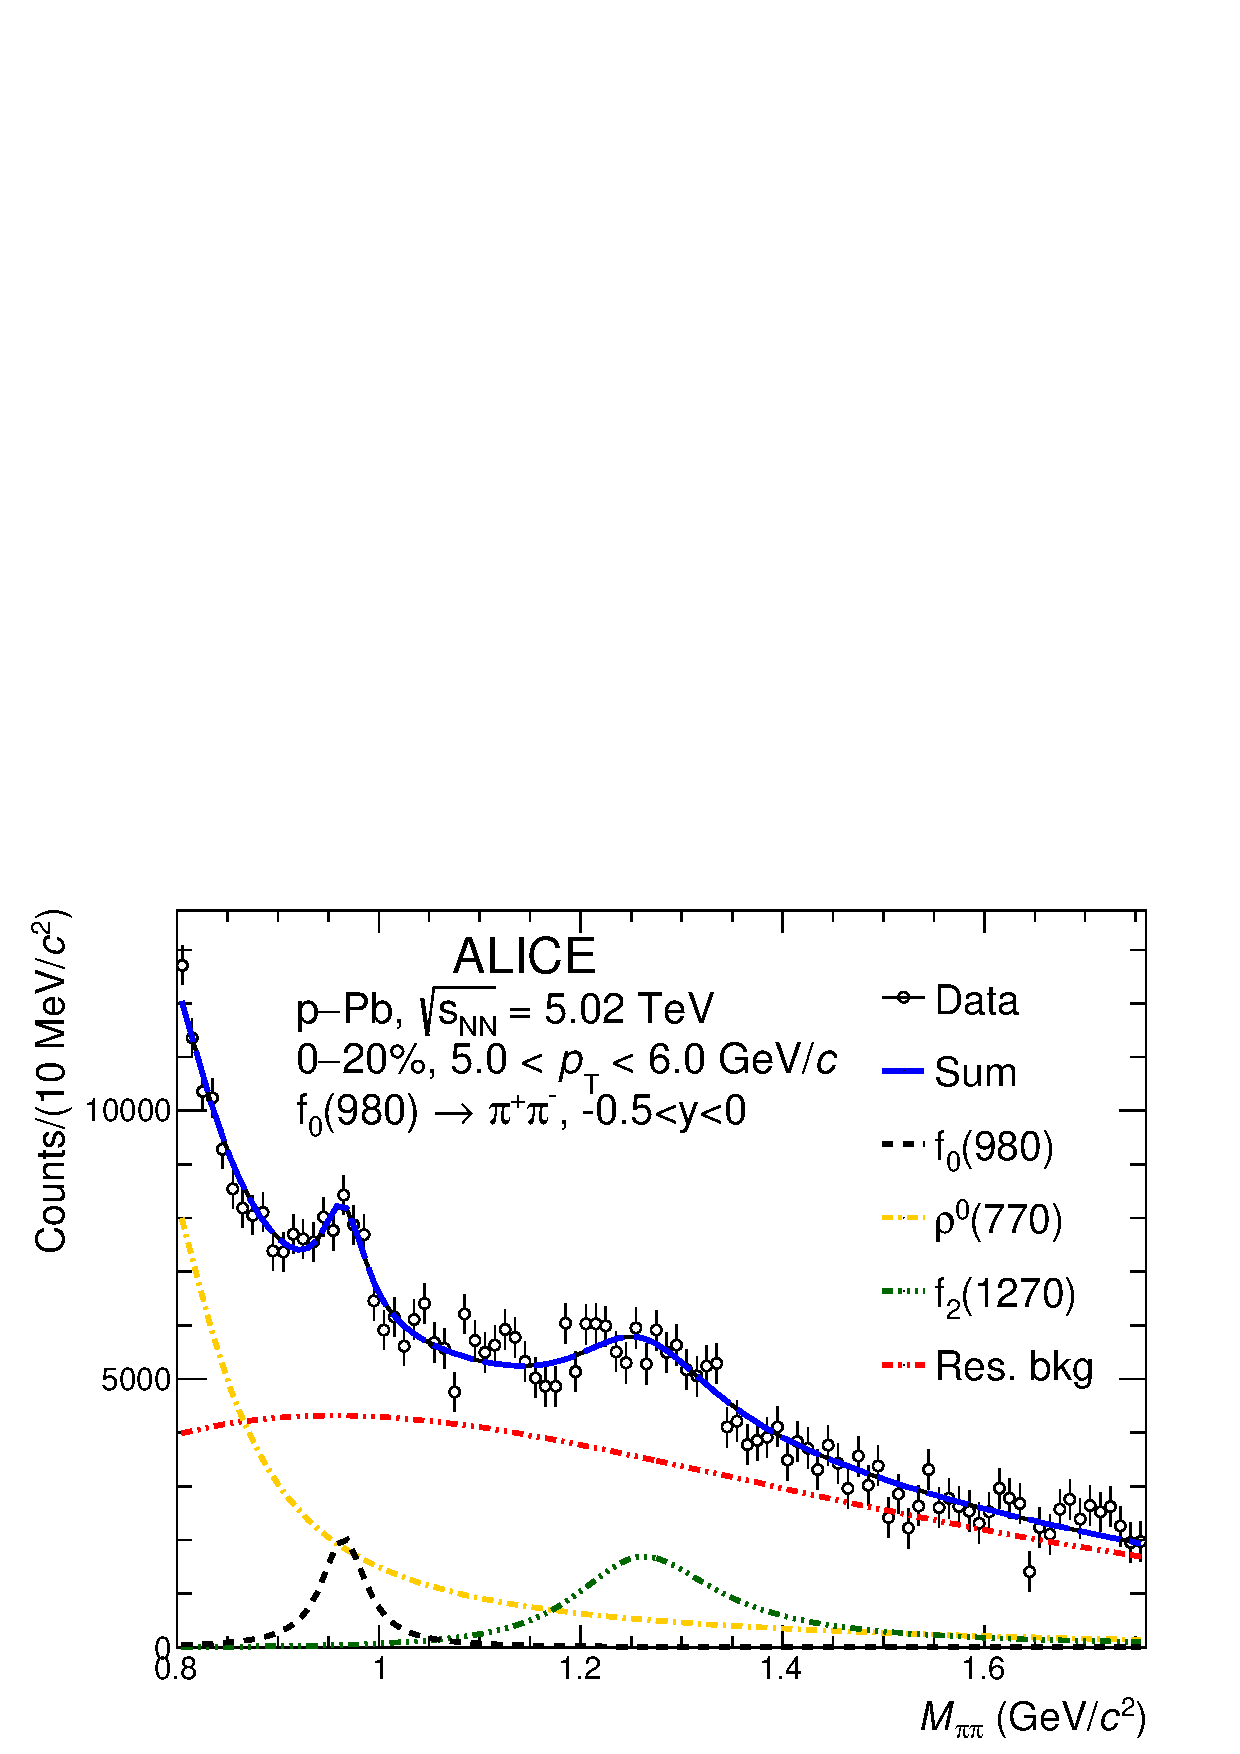
\includegraphics[width=0.47 \textwidth]{figures/Fig1_sigext_high_2pt.pdf} }
	\subfigure{ 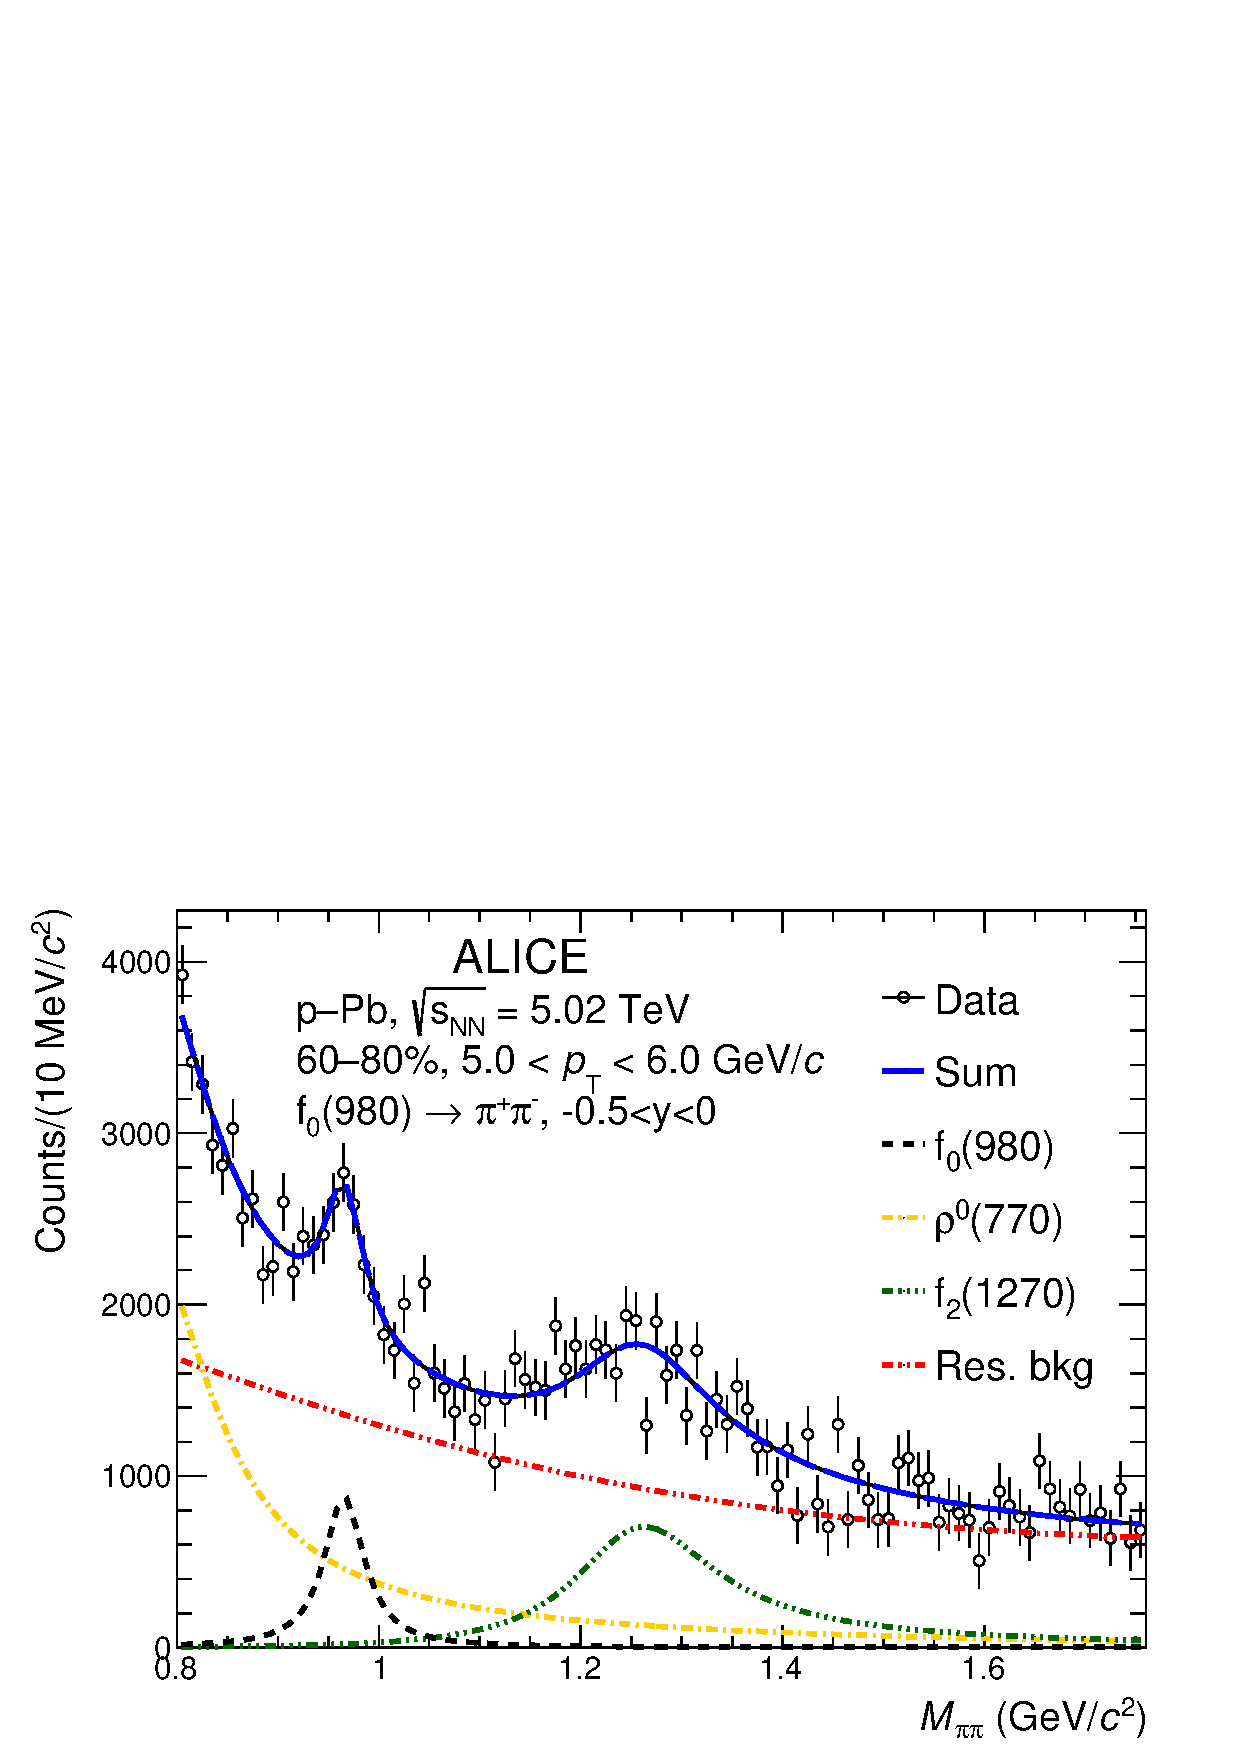
\includegraphics[width=0.47 \textwidth]{figures/Fig1_sigext_low_2pt.pdf} }
	\caption{ Invariant mass distribution of $\pi^{+}\pi^{-}$ pairs after Like-Sign backgrounds subtraction in p--Pb collisions at \snn~=~5.02~TeV in -0.5~$<\mathrm{y}<$~0. Left (Right) plots are obtained from high (low) multiplicity events for different $p_{\mathrm{T}}$ ranges. 
	}
	\label{fig:SigExt}
\end{figure}

The \fzero~is a one of short-lived scalar mesons and its decay vertex is hard to be separated from the primary vertex. The \fzero~is reconstructed with decay channel of \fzero~$\rightarrow \pi^{+}\pi^{-}$, where the branching ratio of the decay is 46\%~\cite{Stone:2013eaa}. The reconstructed tracks are required to satisfy selections listed in the previous work~\cite{ALICE:2018qdv}. The identification of charged pions is done with the TPC and the TOF information. The difference of ionization energy loss between the prediction Bethe-Block parametrization with the pion mass and measured energy is required to be within two standard deviations to identify pions. The difference of flight time between the prediction with the pion mass and measured time is required to be within three standard deviations to identify pions. Identified charged pions are required to be $p_{\rm{T}}>$~0.15~GeV/$c$ and $|\eta|<$~0.8 for a uniform detector acceptance. The pair of two charged pions is required to be -0.5~$<\mathrm{y}<$~0, where $\mathrm{y} = -\mathrm{y}_{\mathrm{lab}} -0.465$~\cite{ALICE:2017pgw}. The combinatorial backgrounds are subtracted with the Like-Sign method~\cite{PhysRevD.36.2019}, which pairs two same charge pions, $\pi^{+}\pi^{+}$ and $\pi^{-}\pi^{-}$. The Like-Sign backgrounds are constructed as the geometric average of $\pi^{+}\pi^{+}$ and $\pi^{-}\pi^{-}$ distributions,  2$\sqrt{N^{\pi^{+}\pi^{+}}N^{\pi^{-}\pi^{-}}}$. After subtracting the Like-Sign backgrounds from $\pi^{+}\pi^{-}$ distribution, peaks of resonances decaying to $\pi^{+}\pi^{-}$ can be seen. Figure~\ref{fig:SigExt} shows the Like-Sign-subtracted $\pi^{+}\pi^{-}$ invariant mass distributions in high-multiplicity (left) and low-multiplicity (right) events for different $p_{\mathrm{T}}$ ranges. Because $\rho$(770) and $\rm{f}_{2}$(1270) dominantly decay to $\pi^{+}\pi^{-}$, \fzero~signals are overlapped with contributions from $\rho$(770) and $\rm{f}_{2}$(1270). Additional backgrounds are attributed to misidentified particles and mini-jets, which are represented as red-dashed-dotted lines in Fig.~\ref{fig:SigExt}. Each resonance contribution is described with relativistic Breit-Wigner function (rBW)~\cite{ALICE:2018qdv, ALICE:2022qnb} because detector resolution is expected to be negligible with respect to the particle width. The rBW can be expressed as
\begin{eqnarray}
\mathrm{rBM}(M_{\pi\pi}) = \dfrac{AM_{\pi\pi}\Gamma(M_{\pi\pi})M_{0}}{(M_{\pi\pi}^{2}-M_{0}^{2})^{2} + M_{0}^{2}\Gamma^{2}(M_{\pi\pi})},
\label{eq:rBW}
\end{eqnarray}
where $\Gamma(M_{\pi\pi})$ is
\begin{eqnarray}
\Gamma(M_{\pi\pi}) = \left[ \dfrac{ (M_{\pi\pi}^{2} - 4m_{\pi}^{2}) }{ (M_{0}^{2}-4m_{\pi}^{2}) } \right]^{(2J+1)/2} \times \dfrac{\Gamma_{0}M_{0}}{M_{\pi\pi}}
\label{eq:rBWW}
\end{eqnarray}
$A$ and $M_{0}$ in eq~\ref{eq:rBW} are amplitude of the rBW and  the rest mass of the resonance, respectively. $\Gamma_{0}$, $J$, and $m_{\pi}$ the are rest width of the resonance, the spin, and the charged pion mass, respectively. The spin for \fzero~, $\rho$(770), and $\mathrm{f}_{2}$(1270) are 0, 1, and 2, respectively. Residual backgrounds ($f_{\mathrm{bkg}}$) is expressed with a similar function with the Maxwell-Boltzmann distribution, which can be expressed as~\cite{OPAL:1998enc}
\begin{eqnarray}
f_{\mathrm{bkg}}(M_{\pi\pi}) = B(M_{\pi\pi}-2m_{\pi})^{n}\exp{(c_{1}M_{\pi\pi} + c_{2}M_{\pi\pi}^{2})}.
\label{eq:bkg}
\end{eqnarray} 
Each rBW of the resonance is corrected for phase space, a mass dependent reconstruction efficiency and $\pi\pi$ interference as described by~\cite{Rapp:2003ar}, which can be expressed as
\begin{eqnarray}
\mathrm{PS}(M_{\pi\pi}) = \dfrac{M_{\pi\pi}}{\sqrt{M_{\pi\pi}^{2}+p_{\mathrm{T}}^{2}}}\times\exp{(-\sqrt{M_{\pi\pi}^{2}+p_{\mathrm{T}}^{2}})},
\label{eq:ps}
\end{eqnarray} 
where $T$ is the kinetic freeze-out temperature and set to 160~MeV~\cite{ALICE:2013wgn} for different multiplicity classes.

The signal extraction carefully considers the width of \fzero~as the width is not constrained (10~$<\Gamma_{\mathrm{f}_{0}}<$~100~MeV/$c^{2}$~\cite{ParticleDataGroup:2020ssz}). Total fit function consists of three rBWs and $f_{\mathrm{bkg}}$, which is constructed with 9 fit parameters as the masses and widths of $\rho$(770) and $\mathrm{f}_{2}$(1270) are well defined in~\cite{ParticleDataGroup:2020ssz}, and those are fixed. The first fit procedure is only conducted in minimum-bias events for merged $p_{\mathrm{T}}$ ranges to accumulate enough statistics while all parameters are left free to obtain unbiased \fzero~width. The second fit procedure is conducted with the fixed \fzero~width, which is obtained from the first procedure, and no constraints for other parameters. As a result of the second procedure, four parameters of backgrounds function are determined. The last fit procedure is conducted with the fixed background function, and no constraints for other parameters. In each step, the fit range is set to 0.8~$<M_{\pi\pi}<$~1.76~GeV/$c^{2}$. Such multiple steps are designed to prevent fit results from being in local minimum and to minimize possible biases to the estimation of the \fzero~width. 

Raw \fzero~yields from fit procedures are corrected for the acceptance and the tracking efficiency, and normalized for the event selections and the branching fraction~\cite{ALICE:2022qnb}. Coefficients for the accepance and the tracking efficiency are estimated from a detailed simulation for the ALICE detector responses. The p--Pb events are simulated using the DPMJET~\cite{Fedynitch:2015kcn} event generator with the artificial injection of \fzero~signals. The generated \fzero~are transported through the detector using GEANT3~\cite{Brun:1994aa}. The acceptance multiplied by the tracking efficiency is estimated to be 26\% and gradually increasing up to 60\% as $p_{\mathrm{T}}$ increases. 

A comparison of the $p_{\rm{T}}$ differential invariant yield between p--Pb and pp collisions, which is called the nuclear modification factor ($Q_{\mathrm{pPb}}$), can be expressed as
\begin{eqnarray}
Q_{\mathrm{pPb}} = \dfrac{\mathrm{d}^{2} N_{\mathrm{f}_{0}(980)}^{\mathrm{pPb}} / \mathrm{d} p_{\mathrm{T}} \mathrm{dy} }{ \left\langle T_{\mathrm{pPb}} \right\rangle \mathrm{d}^{2} \sigma_{\mathrm{f}_{0}(980)}^{\mathrm{pp}}/ \mathrm{d} p_{\mathrm{T}} \mathrm{dy} },
\end{eqnarray}
where $\left\langle T_{\mathrm{pPb}} \right\rangle$ and $\sigma_{\mathrm{f}_{0}(980)}^{\mathrm{pp}}$ are the average nuclear overlap from the Glauber model~\cite{Miller:2007ri} and the cross section of \fzero~in pp collisions~\cite{ALICE:2022qnb}, respectively. 

\section{Systematic uncertainties}
\label{sec:syst}
The systematic uncertainties of invariant yields are estimated by varying the analysis selection criteria and corrections, which are summarized in Tab.~\ref{tab:syst}. Total systematic uncertainty is calculated as a quadrature of each uncertainty.

\begin{table}[h!]
\caption{The relative systematic uncertainty of invariant $p_{\rm{T}}$-differential yields. Numbers given in ranges correspond to minimum and maximum uncertainties.}
\centering
\begin{tabular}{cc|c}
\hline 
\multicolumn{2}{c|}{Sources}  &Systematic uncertainty (\%) \\ \hline
\multicolumn{2}{c|}{Tracking} & $\pm$4--6 \\
\multicolumn{2}{c|}{Particle identification} & $\pm$4--12 \\ 
\multirow{4}{*}{Signal extraction} &  $\mathrm{f}_{2}$(1270) Par.	& $\pm$3--9 \\ 
& $\rho$(770) Par. & $\pm$3--8 \\
& Fit range & $\pm$0--6 \\
& Init. $\mathrm{f}_{0}$ width & $\pm$2--12 \\
\multicolumn{2}{c|}{Phase space correction} & $\pm$3--8 \\ \hline 
\multicolumn{2}{c|}{Total (in quadrature)}	& $\pm$15--27 \\ 
\hline 
\end{tabular}
\label{tab:syst}
\end{table}

The systematic uncertainty from the primary vertex selection is tested by narrowing the requirement to 7~cm and the uncertainty is estimated to be negligible. The systematic uncertainty from the pileup rejection is tested by varying the minimal number of track contributors required for reconstruction of pileup event vertices from 5 to 3 and the uncertainty is estimated to be negligible.

The systematic uncertainty from tracking is assigned as the value from~\cite{ALICE:2013wgn} and the systematic uncertainty from the particle identification is tested with different requirements on the number of standard deviations by $\pm\,0.5\sigma$ for the TPC and the TOF, and the uncertainties are estimated to be 4--12\%.

The systematic uncertainties from masses and widths of $\mathrm{f}_{2}$(1270) and $\rho$(770) are evaluated by shifting the masses and the widths as much as three times their measured statistical uncertainty. The estimated uncertainties from $\mathrm{f}_{2}$(1270) and $\rho$(770) parameters are 3--9\% and 3--8\%, respectively. The systematic uncertainty from the fit range is estimated by changing the range inward or outward as much as 40~MeV/$c^{2}$. The uncertainties are estimated to be 0--6\%.

The systematic uncertainty from the initial \fzero~width, which is obtained in the first fit procedure and used in the second fit procedure (see Sec.~\ref{sec:ana}), is estimated by varying the width as much as their measured statistical uncertainty in both directions. The estimated systematic uncertainties are 2--12\%.

The systematic uncertainty from phase space correction is estimated by varying the kinetic freeze-out temperature in the range of 140~$<T_{\mathrm{kin}}<$~180~MeV. The estimated uncertainty is 3--8\%. 

\begin{comment}
The systematic uncertainties of invariant yields and \fzero~widths are estimated by varying the analysis selection criteria and corrections, which are summarized in Tab.~\ref{tab:syst}.

The systematic uncertainty from the primary vertex selection is tested by narrowing the requirement to 7~cm and the uncertainty is estimated to be negligible. The systematic uncertainty from the pileup rejection is tested by varying the minimal number of track contributors required for reconstruction of pileup event vertices from 5 to 3 and the uncertainty is estimated to be negligible.

The systematic uncertainty from tracking is assigned as the value from~\cite{ALICE:2013wgn} and the systematic uncertainty from the particle identification is tested with different requirements on the number of standard deviations by $\pm\,0.5\sigma$ for the TPC and the TOF, and the uncertainties are estimated to be 4--12\% for invariant yield and 5--10\% for width.

The systematic uncertainties from masses and widths of $\mathrm{f}_{2}$(1270) and $\rho$(770) are evaluated by shifting the masses and the widths as much as three times their measured statistical uncertainty. The estimated uncertainties for $\mathrm{f}_{2}$(1270) ($\rho$(770)) parameters are 3--9\% (3--8\%) and 2--7\% (2--8\%) for the mass and the width, respectively. The systematic uncertainty from the fit range is estimated by changing the range inward or outward as much as 40~MeV/$c^{2}$. The uncertainties are estimated to be 0--6\% for the yield and 0--5\% for the width.

On the other hand, the width of \fzero~is loosely defined so that \fzero~width is set to free parameter and estimated in the fit procedure. The systematic uncertainty from the fit range is tested with different fit ranges and estimated to be 2\% at the low $p_{\rm{T}}$ and 8\% at the high $p_{\rm{T}}$. The phase space correction~\cite{Rapp:2003ar} is applied to each rBW to consider possible $\pi\pi$ scattering effects. The temperature of the phase space correction is set to 160 MeV~\cite{ALICE:2013wgn} and the systematic uncertainty from the phase space correction is evaluated with different temperatures and estimated to be 5--7\%. The background function is determined with the pre-fit procedure. In the pre-fit procedure, the width of \fzero~is even fixed as a specific value. The systematic uncertainty from the background function is evaluated with different \fzero~widths and estimated to be 8\% at the low $p_{\rm{T}}$ and 3\% at the high $p_{\rm{T}}$.
\end{comment}
% !TEX root = paper.tex

\section {Results}
\label{sec:results}

\begin{figure}[!hbt]
	\centering
	\subfigure{ 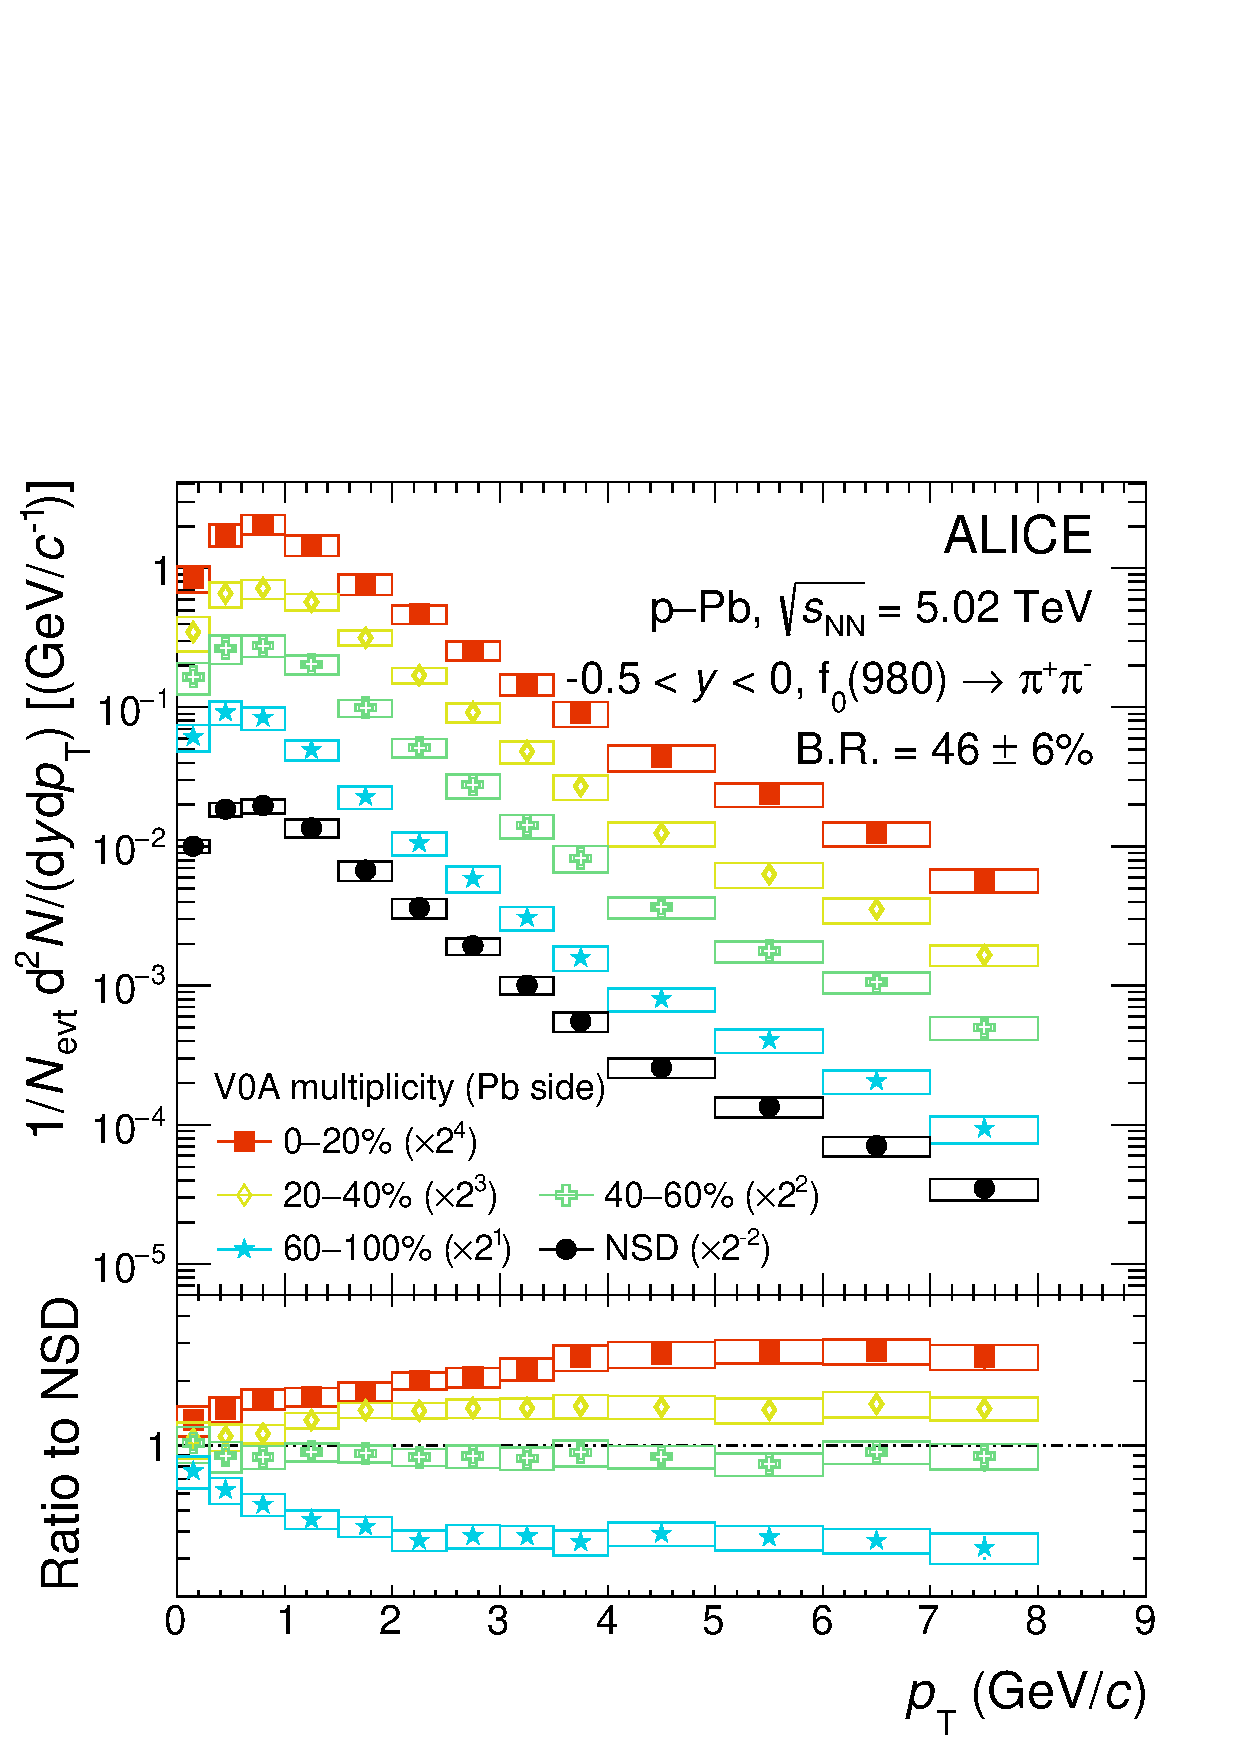
\includegraphics[width=0.6 \textwidth]{figures/Fig2_pt_all.pdf} }
	\caption{ Transverse momentum spectra of \fzero~in p--Pb collisions at \snn~=~5.02~TeV for different multiplicity classes, which are scaled for visibility. Statistical and systematic uncertainties are shown as error bars and boxes, respectively. The lower panel shows the ratios of the specific spectra to the minimum-bias NSD spectrum. }
	\label{fig:pt}
\end{figure}

Figure~\ref{fig:pt} shows the $p_{\mathrm{T}}$ spectra of \fzero~in p--Pb collisions at \snn~=~5.02~TeV measured in the range of 0~$<p_{\mathrm{T}}<$~8~GeV/$c$ for different multiplicity classes. Each spectrum is scaled with the number denoted in the figure for visibility. The lower panel of Fig.~\ref{fig:pt} shows the ratios of each $p_{\mathrm{T}}$ spectrum to the minimum-bias $p_{\mathrm{T}}$ spectrum. Increasing mean $p_{\mathrm{T}}$ are observed with the increasing multiplicity.

\begin{figure}[!hbt]
	\centering
	\subfigure{ 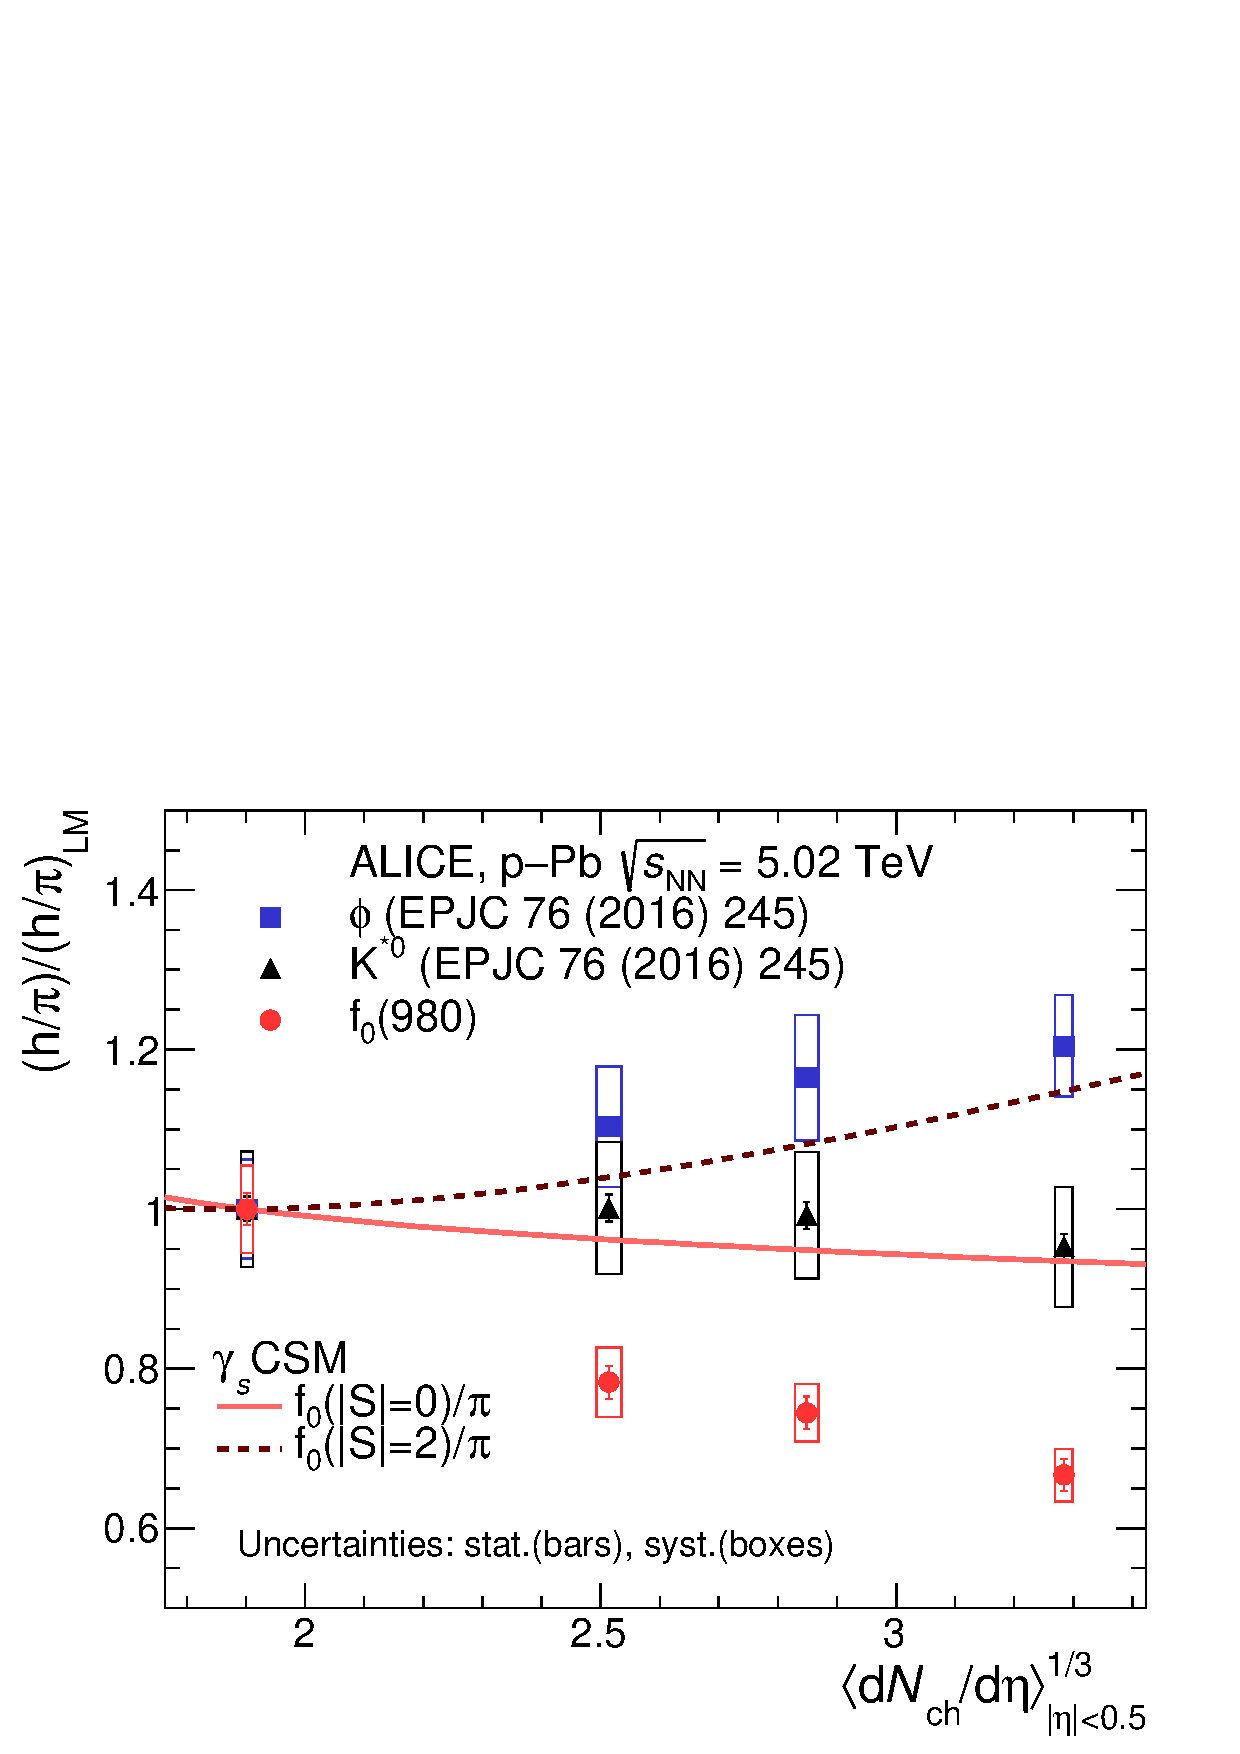
\includegraphics[width=0.6 \textwidth]{figures/Fig4_dr_pion_addCSM.pdf} }
	\caption{ Double ratio of $\phi$, $\rm{}K^{*0}$(892), and \fzero~to $\pi$ as a function of charged-particle multiplicity elevated to 1/3. The ratios are divided by the ratio in low-multiplicity events to make the first point unity. Predictions from Canonical statistical model are represented with solid lines. }
	\label{fig:f0piAddCSM}
\end{figure}

Figure~\ref{fig:f0piAddCSM} shows the double ratios of different particles to charged pion yields as a function of charged-particle multiplicity elevated to 1/3 in p--Pb collisions at \snn~=~5.02~TeV. The ratio of $\phi$ to $\pi$ is increasing with the multiplicity, which favors the observation of the strangeness enhancement~\cite{ALICE:2016fzo}. The ratio of $\rm{}K^{*0}$ to $\pi$ is flat with the increasing multiplicity even $\rm{}K^{*0}$ includes one strange quark. The flat trend is due to the two competing effects, the strangeness enhancement and rescattering effects, as the lifetime of $\rm{}K^{*0}$ is 4.2~fm/$c$~\cite{ParticleDataGroup:2020ssz}. The ratio of \fzero~to $\pi$ is decreasing as the multiplicity increases because of the short lifetime of \fzero, which suggests non-negative rescattering effects for \fzero. Predictions of the ratio of \fzero~to $\pi$ are shown in lines for different hidden strangeness assumptions for \fzero~by Canonical Statistical Model (CSM)~\cite{Vovchenko:2019kes}. The CSM with two hidden strangeness estimates the ratio to be increasing, which is opposite trend of the experimental result. Moreover, the CSM with zero hidden strangeness estimates the ratio to be flat, which also overestimates the data. The overestimation is attributed to no recattering effects in the CSM.

\begin{figure}[!hbt]
	\centering
	\subfigure{ 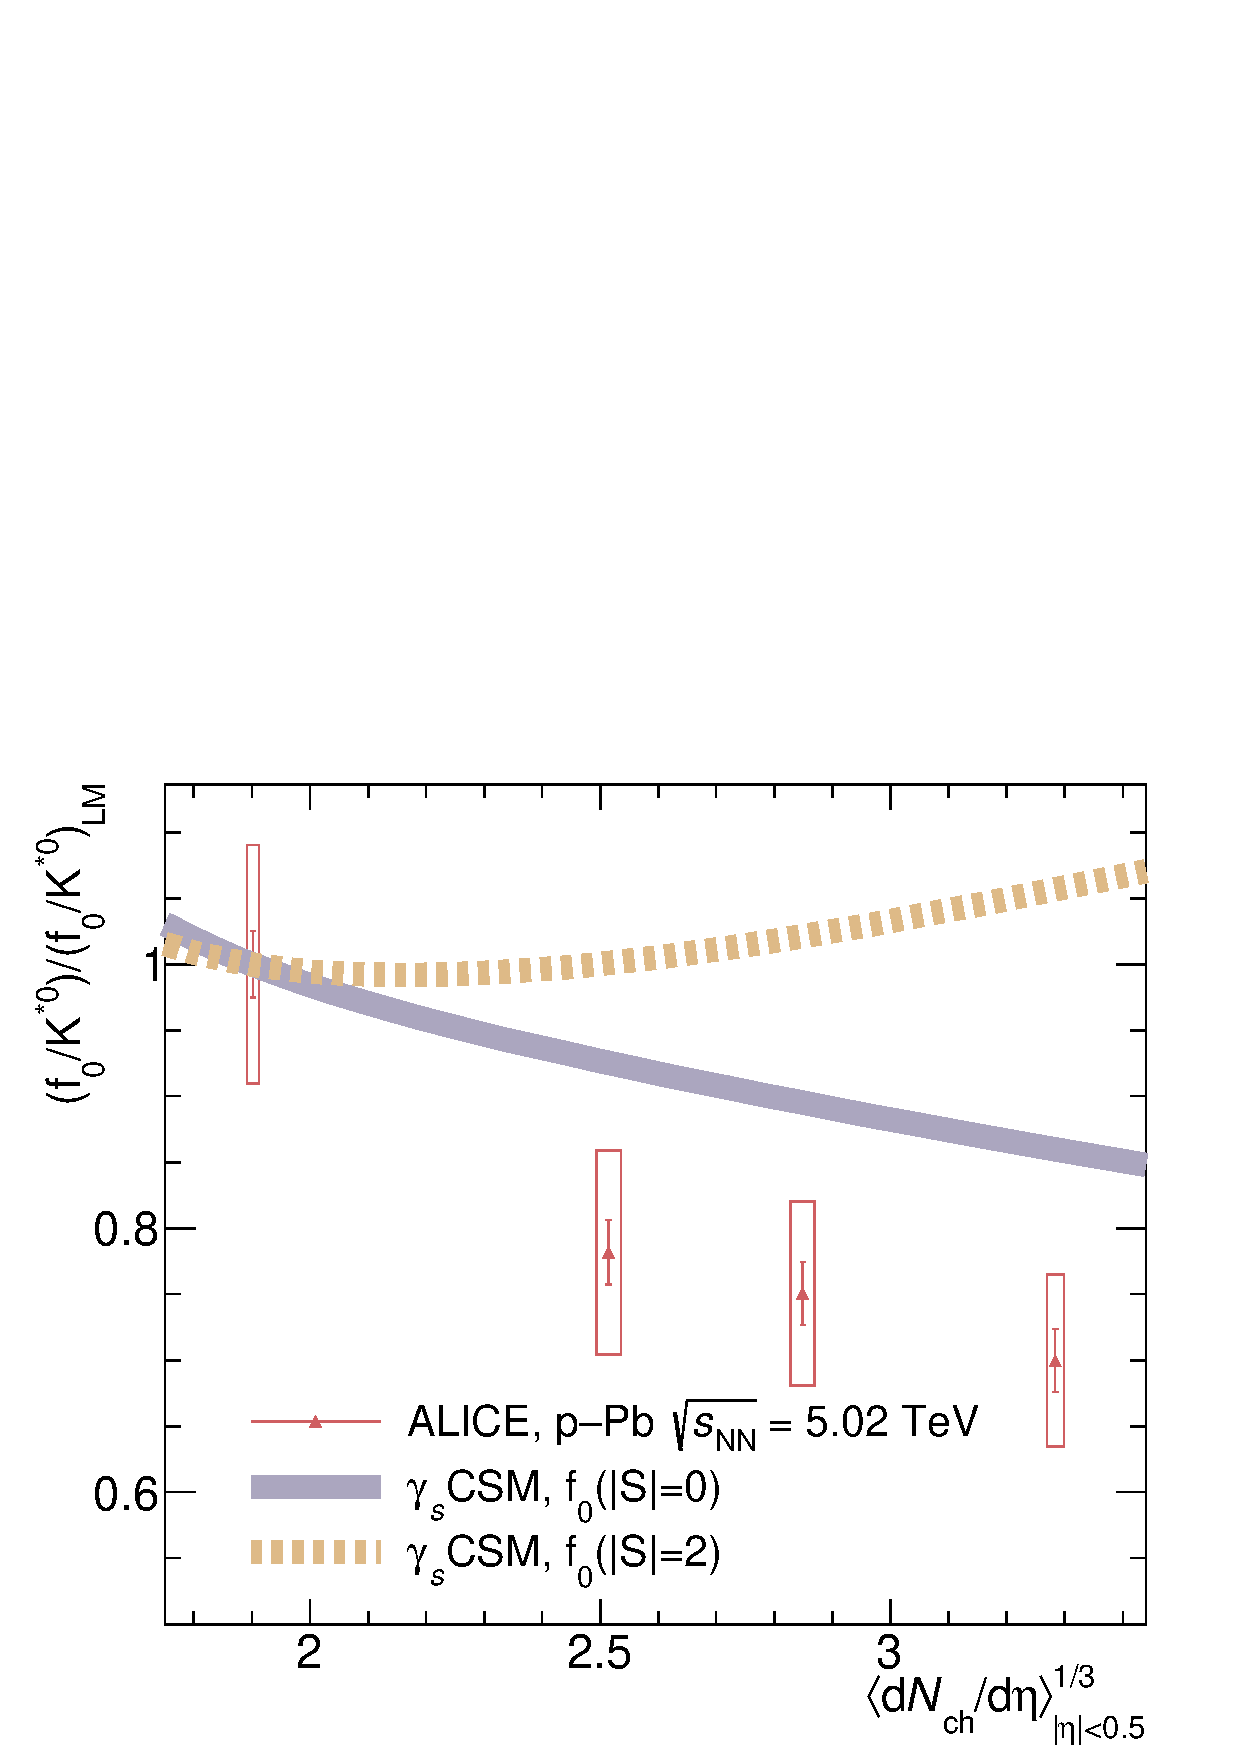
\includegraphics[width=0.6 \textwidth]{figures/Fig4_dr_kstar_addCSM.pdf} }
	\caption{ Double ratio of \fzero~to $\rm{}K^{*0}$ yields as a function of charged-particle multiplicity elevated to 1/3. The ratios are divided by the ratio in low-multiplicity events to make the first point unity. Predictions from Canonical statistical model are represented with solid lines. }
	\label{fig:f0KSAddCSM}
\end{figure}

Figure~\ref{fig:f0KSAddCSM} shows the double ratio of \fzero~to $\rm{}K^{*0}$ yields as a function of charged-particle multiplicity elevated to 1/3 in p--Pb collisions at \snn~=~5.02~TeV and predictions from the CSM with different hidden strangeness assumptions. The ratio is decreasing with the increasing multiplicity, and this trend is qualitatively described with the zero hidden strangeness assumption. The lifetimes of \fzero~and $\rm{}K^{*0}$ are estimated to be comparable, indicating that rescattering effects would not be much different. Hence, the decreasing trend of the ratio is weakly affected by rescattering effects. The CSM prediction with two hidden strangeness assumption is mildly increasing as the multiplicity increases, which is also opposite to the experimental result. Therefore, decreasing trend of the ratio of \fzero~to $\rm{}K^{*0}$ can suggest absence of the strange quark in \fzero.

\begin{figure}[!hbt]
	\centering
	\subfigure{ 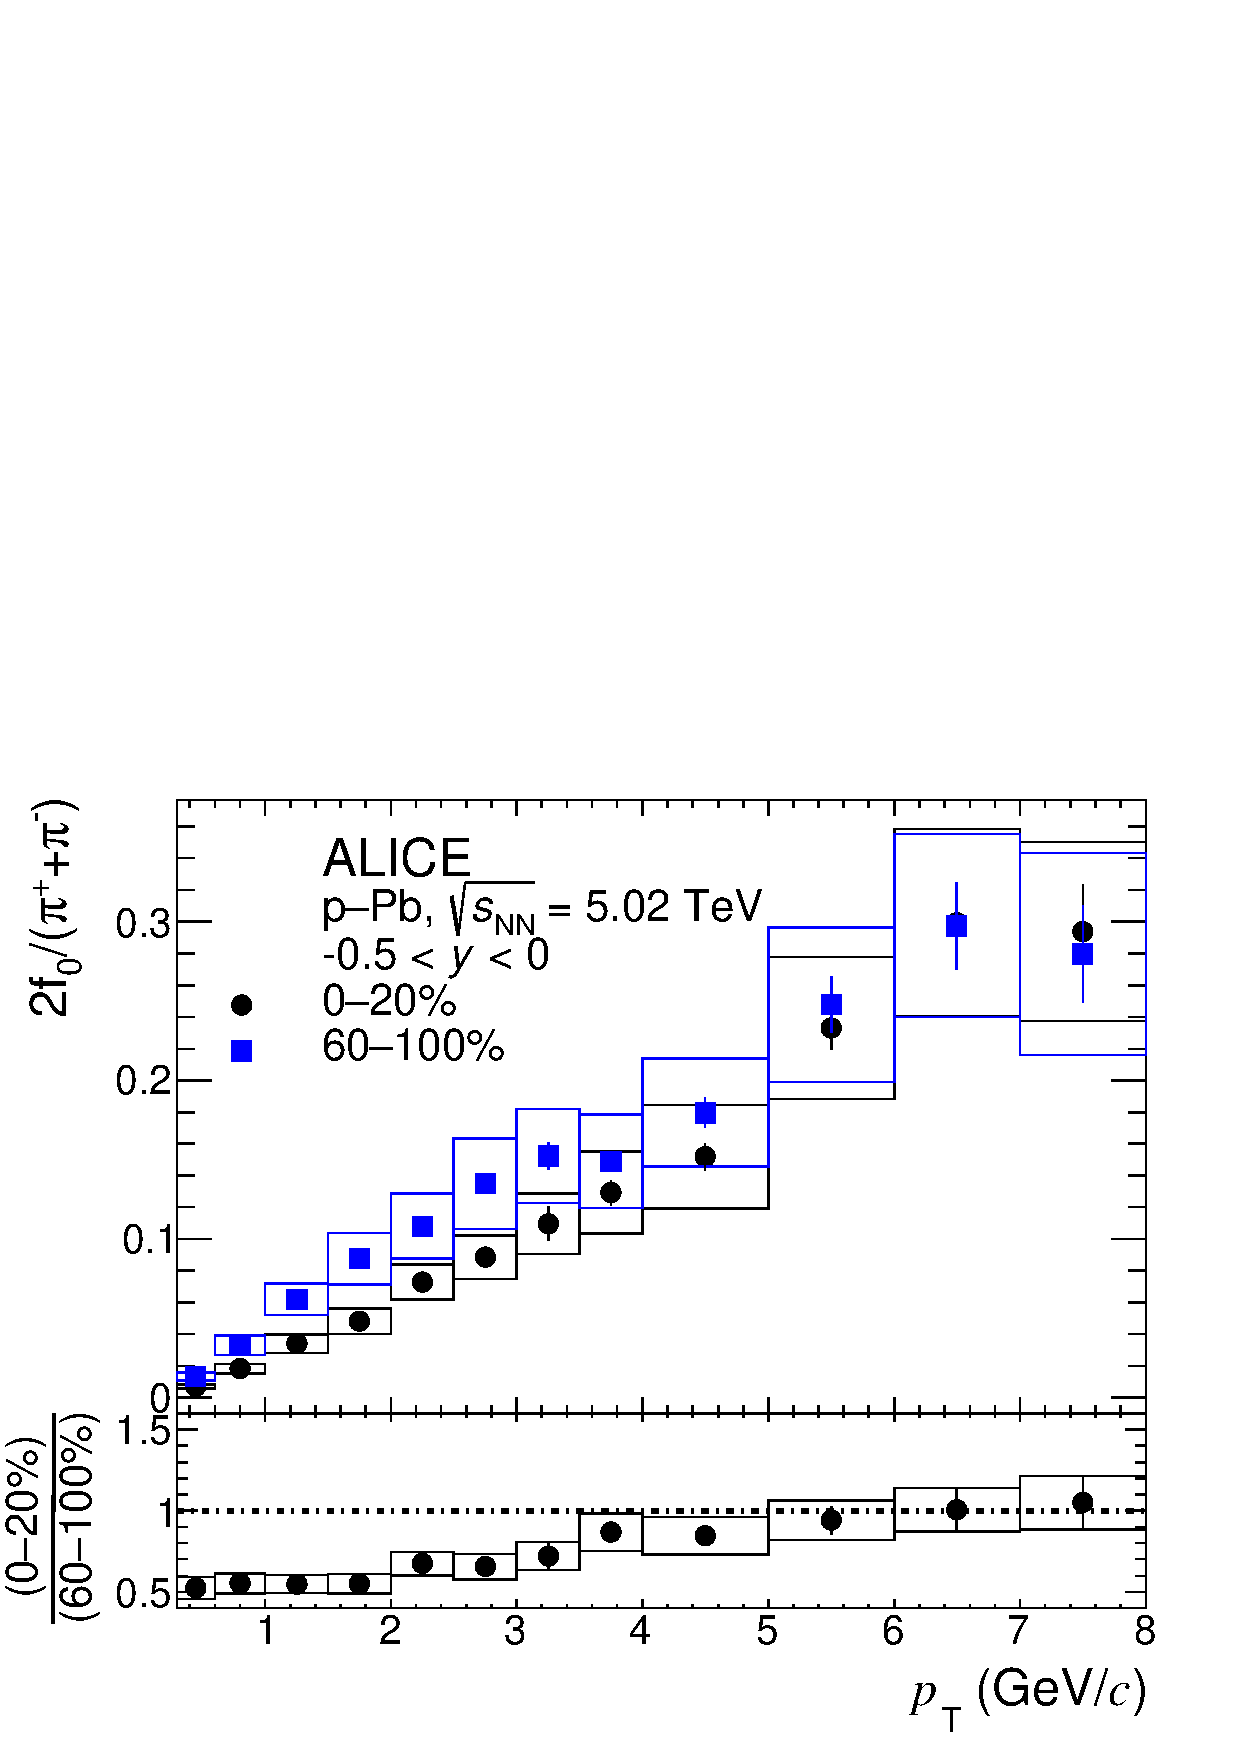
\includegraphics[width=0.6 \textwidth]{figures/Fig5_DR_pt_pion.pdf} }
	\caption{ Particle yield ratio of \fzero~to $\pi$ as a function of $p_{\rm{T}}$ in high-multiplicity (circles) and low-multiplicity (triangles) p--Pb collisions at \snn~5.02~TeV. The lower panel shows the double ratio of high-multiplicity to low-multiplicity \fzero/$\pi$. }
	\label{fig:f0piPt}
\end{figure}

Figure~\ref{fig:f0piPt} shows $p_{\mathrm{T}}$-differential particle yield ratio of \fzero~to $\pi$ in high-multiplicity (HM) and low-multiplicity (LM) p--Pb collisions at \snn~=~5.02~TeV. The ratios are consistent within one sigma for $p_{\mathrm{T}}>$~4~GeV/$c$, while the double ratio of HM to LM is suppressed at low $p_{\mathrm{T}}$, which is shown in the lower panel of Fig.~\ref{fig:f0piPt}. The $p_{\mathrm{T}}$ dependence of the double ratio indicates that the suppression of the integrated yield is a low-$p_{\mathrm{T}}$ effect, which is the qualitatively same $p_{\mathrm{T}}$ dependence as the suppression of the $\rm{}K^{*0}/K$~\cite{ALICE:2019etb}.

\begin{figure}[!hbt]
	\centering
	\subfigure{ 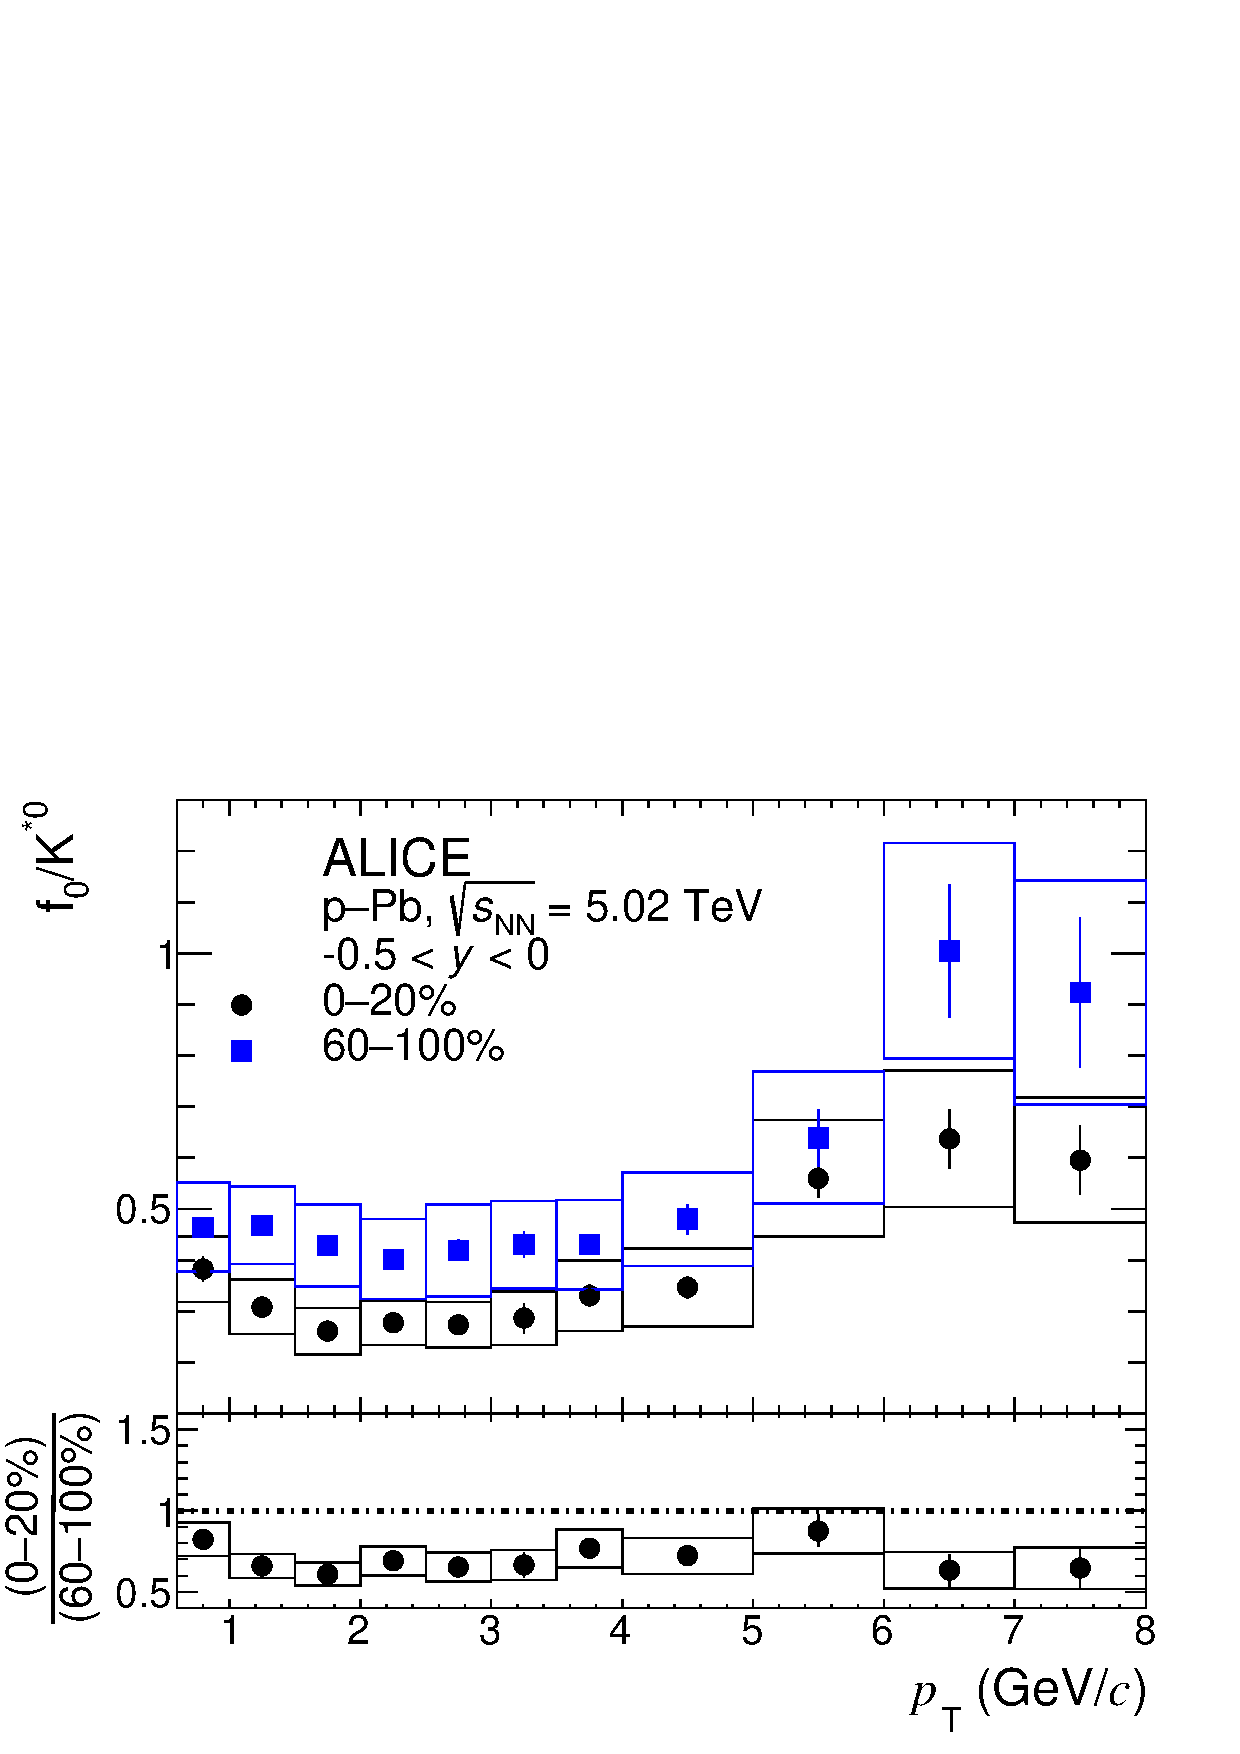
\includegraphics[width=0.6 \textwidth]{figures/Fig6_DR_pt_kstar.pdf} }
	\caption{ Particle yield ratio of \fzero~to $\rm{}K^{*0}$(892) as a function of $p_{\rm{T}}$ in high-multiplicity (circles) and low-multiplicity (triangles) p--Pb collisions at \snn~5.02~TeV. The lower panel shows the double ratio of high-multiplicity to low-multiplicity \fzero/$\rm{}K^{*0}$(892).  }
	\label{fig:f0KsPt}
\end{figure}

Figure~\ref{fig:f0KsPt} shows $p_{\mathrm{T}}$-differential particle yield ratio of \fzero~to $\rm{}K^{*0}$ in HM and LM p--Pb collisions at \snn~=~5.02~TeV. The ratio from HM events is suppressed in the measured entire $p_{\mathrm{T}}$ range, which is significantly different from the $p_{\mathrm{T}}$ dependence of $\rm{}K^{*0}/K$ or \fzero/$\pi$. The different $p_{\mathrm{T}}$ dependence of the double ratio indicates that the other effects, rather than rescattering effects, are present. For instance, the enhancement of $\rm{}K^{*0}$ yield due to the strangeness enhancement can explain the suppression at the entire $p_{\mathrm{T}}$ range. As a result, the relative suppression suggests no strange quark in \fzero.

\begin{figure}[!hbt]
	\centering
	\subfigure{ 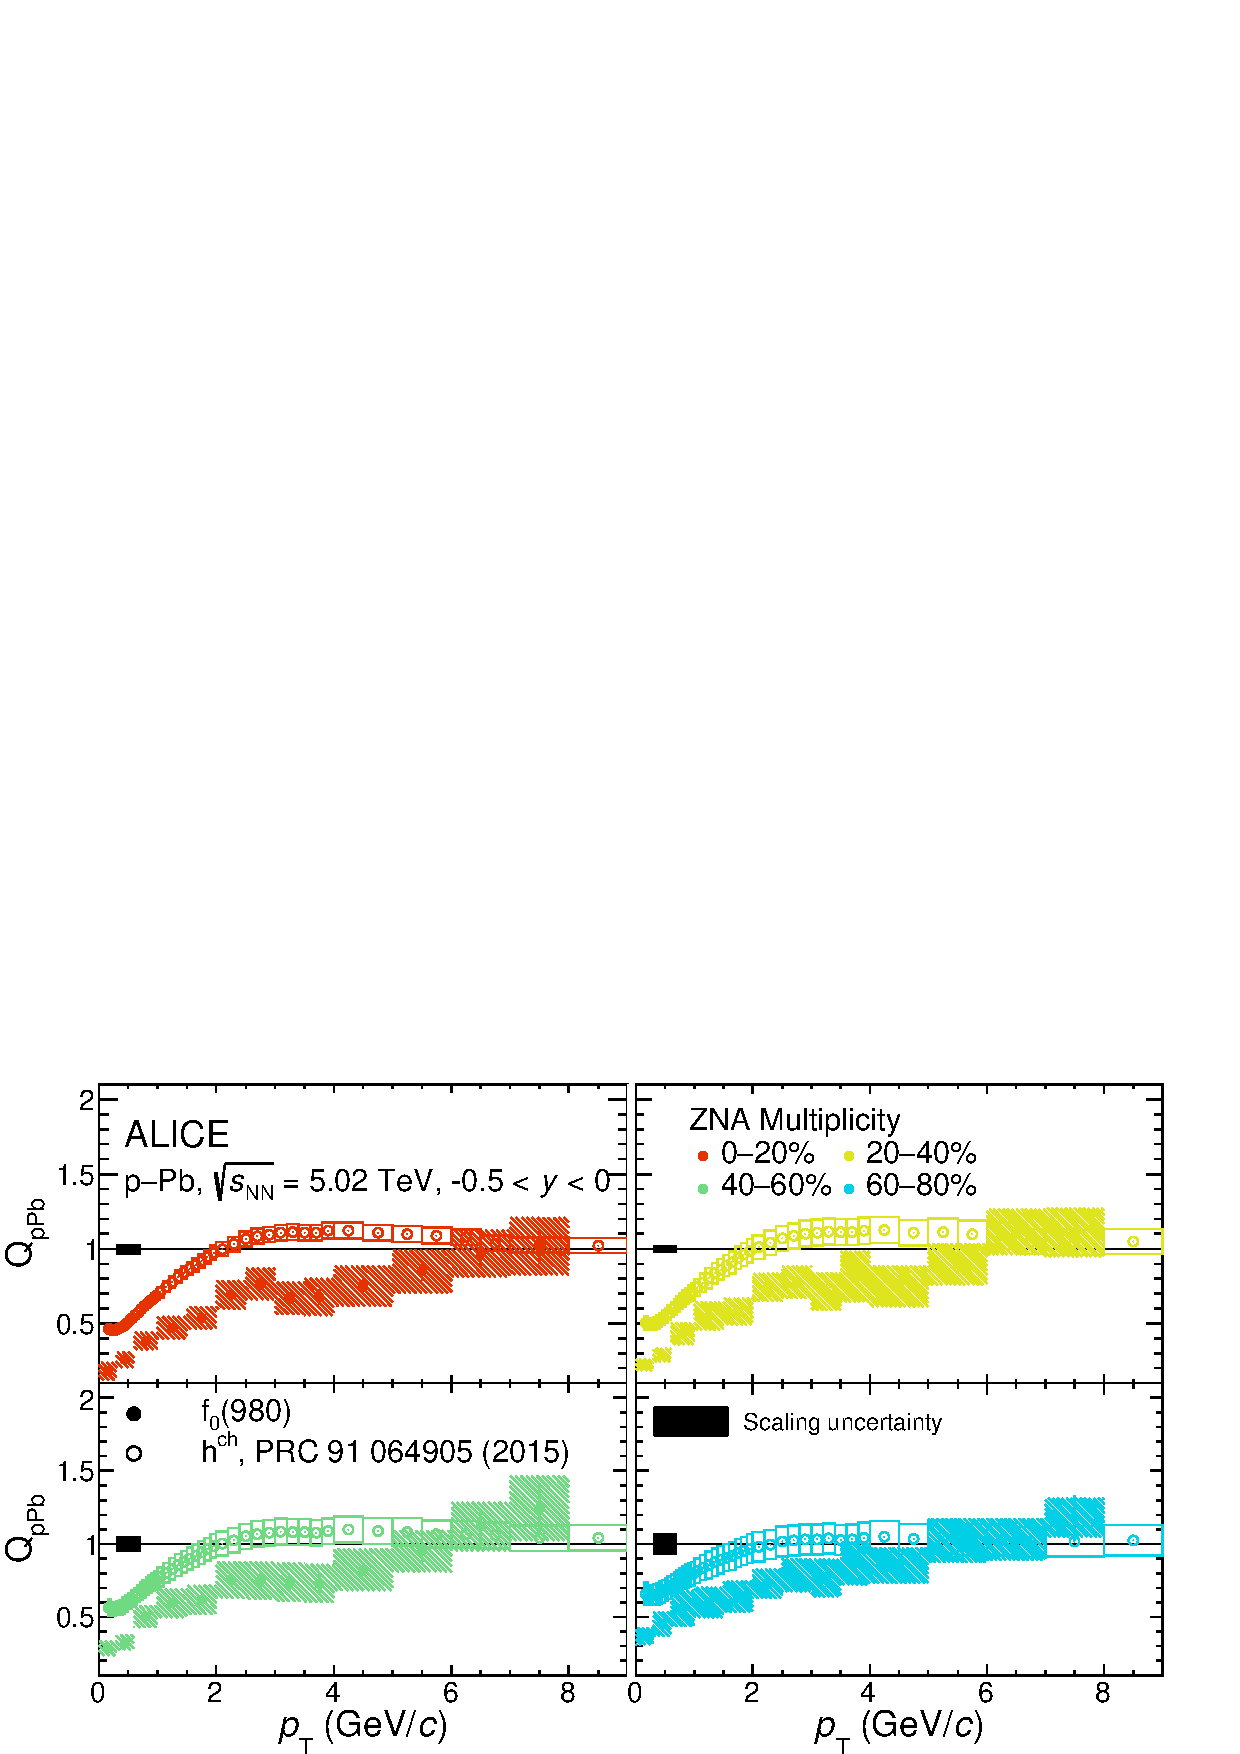
\includegraphics[width=0.8 \textwidth]{figures/Fig7_QpPb.pdf} }
	\caption{ Nuclear modification factor ($Q_{\rm{pPb}}$) of \fzero~as a function of $p_{\rm{T}}$ in p--Pb collisions at \snn~5.02~TeV for different multiplicity classes. Statistical and systematic uncertainties are shown as error bars and boxes, respectively. Open boxes around $p_{\rm{T}}$~=~0.5~GeV/$c$ represent the binary collision scaling uncertainties. The $Q_{\rm{pPb}}$ of \fzero~is compared with \fzero~of charged hadrons. }
	\label{fig:QpPb}
\end{figure}

Figure~\ref{fig:QpPb} shows the nuclear modification factor ($Q_{\rm{pPb}}$) of \fzero~in p--Pb collisions at \snn~=~5.02~TeV in different multiplicity classes. The systematic uncertainties are calculated with the assumption that there is no correlated uncertainty between the cross section in pp and p--Pb collisions. The \fzero~is much suppressed than charged hadrons in all measured centrality intervals for $p_{\mathrm{T}}<$~4~GeV/$c$. As $p_{\mathrm{T}}$ increases, the difference of $Q_{\rm{pPb}}$ gets smaller. The observation can be also related to the existence of rescattering effects for \fzero. In addition, the $Q_{\rm{pPb}}$ does not exhibit Cronin peak~\cite{Cronin:1974zm} at the intermediate $p_{\mathrm{T}}$ in HM events, while all baryons do. No Cronin peak for \fzero~might suggest the number of constituent quarks of \fzero~to be smaller than three.
% !TEX root = paper.tex

\section{Conclusions}
\label{sec:summary}

The multiplicity and $p_{\mathrm{T}}$ dependence of \fzero~production in p--Pb collisions at \snn~=~5.02~TeV is presented. The \fzero~is reconstructed via the \fzero~$\rightarrow\pi^{+}\pi^{-}$ decay channel at midrapidity ($-0.5<y<0$) in the transverse momentum region of $0<p_{\mathrm{T}}<8$~GeV/$c$. A hardening of the $p_{\mathrm{T}}$ spectra and a consequent increase of the mean $p_{\mathrm{T}}$ are observed with increasing multiplicity. The $p_{\mathrm{T}}$-integrated particle yield ratio of \fzero~to $\pi$ is decreasing with increasing multiplicities, and the $p_{\mathrm{T}}$-differential studies show a clear suppression of the \fzero~to $\pi$ ratio for $p_{\mathrm{T}}<$~3.5~GeV/$c$, indicating that rescattering effects for \fzero~particles exist in p--Pb collisions. The CSM overestimates the \fzero/$\pi$ ratio, and it does not describe the decreasing trend because the CSM does not consider rescattering processes. The $p_{\mathrm{T}}$-integrated \fzero/\kstar~yield ratio also decreases with increasing multiplicity. The suppression of the \fzero~to \kstar~ratio is observed in the entire measured $p_{\mathrm{T}}$ range, showing a different $p_{\mathrm{T}}$ dependency relative to the one expected from a rescattering scenario. The CSM qualitatively describes the decreasing trend for the $p_{\mathrm{T}}$-integrated \fzero/\kstar~ratio as a function of multiplicity with the assumption of no hidden strangeness for \fzero, while it overestimates the \fzero/\kstar~with the assumption of two strange quarks. These results indicate that the production of \kstar~is relatively enhanced compared with \fzero~due to the strangeness enhancement. Additionally, $p_{\mathrm{T}}$-differential \fzero/\kstar~ratio does not exhibit the enhancement of baryon-to-meson ratio, suggesting the number of constituents quarks for \fzero~to be two. Furthermore, the multiplicity-dependent nuclear modification factor ($Q_{\mbox{pPb}}$) for \fzero~exhibits a strong suppression at low $p_{\mathrm{T}}$, and the suppression depends on the multiplicity class, which can be explained by the rescattering effects. In addition, no Cronin-like enhancement is observed in $Q_{\mbox{pPb}}$, even in high-multiplicity events. The absence of the Cronin-like enhancement suggests that the number of constituent quarks of the \fzero~particle is two. The abnormal suppression in terms of multiplicity and transverse momentum relative to other particles sheds light on the internal structure of \fzero~to be a conventional meson and provides insight into the properties of the late hadronic phase in p--Pb collisions.




%%%%% acknowledgements
\newenvironment{acknowledgement}{\relax}{\relax}
\begin{acknowledgement}
\section*{Acknowledgements}
\noindent 
%{\it (TBI: The default acknowledgments will be done by EB centrally.)}
%\input{acknowledgements.tex}    %%%%%%% done by webmaster team
\end{acknowledgement}

\newpage
\appendix



\clearpage

\bibliographystyle{utphys}
\bibliography{paper.bib}

%%%%%%%%% appendix with author list
%\section{The ALICE Collaboration}
%\label{app:collab}
%\input{Alice_Authorlist_2017-Aug-21.tex}  %%%%%%% done by webmaster team
%\input{}     


\end{document}
